\documentclass[12pt, titlepage]{report}
\usepackage[T1]{fontenc}
\usepackage{hyperref}
\usepackage[utf8]{inputenc}
\usepackage[english]{babel}
\usepackage{amsmath}
\usepackage{amsthm}
\usepackage{amssymb}
\usepackage{amsfonts}
\usepackage{mathtools}
\usepackage{booktabs}
\usepackage{caption}
\usepackage{subcaption}
\usepackage{graphicx}
\usepackage{float}
\usepackage{multirow}
\usepackage{braket}
\usepackage[nottoc,numbib]{tocbibind}
\usepackage{blindtext}
\usepackage{scrextend}

\title{Foundations of HPC: report of the final assignment}
\author{Giovanni Varutti, Samuele Lippolis}

\begin{document}

\maketitle
\newpage
\tableofcontents
\newpage
		
\chapter{Assignment 1}

	
\section{Introduction}\label{Introduction}

The aim of this assignment is to implement a parallel version of the famous Conway's game of life, with an hybrid openMP and MPI approach for the parallelization.
The Conway's game of life is a cellular automaton which plays autonomously on an infinite 2D grid of cells. The game is then deterministinc and the evolution 
depends only on the initial conditions. The playground is realized with a square grid of size $k\times k$ with periodic boundary conditions at the edges.
The neighbours of a cell are the 8 most adjacent cells, i.e. those that on a grid representation share an edge with the considered cell.
The periodic boundary conditions state that cells at an edge have to be considered neighbours of the cells at the opposite edge along the same axis.
For the evolution of the playground, the following evolution methods have been implemented:
\begin{itemize}
	\item \textbf{Static evolution}: we freeze the whole playground in which each cell is in a state $s_i$. Then we evaluate the next status $s_{i+1}$ of each cell until the last cell, and memorize it. The status update of the playground is done only at the end of the computation of the status evaluation.
	\item \textbf{Ordered evolution}: the next status of a certain cell is evaluated and immediately updated. This is done sequencially for each cell following the rows order, and starting from the cell $(0,0)$ in the top left corner. This obviously introduce a spurious signal through the playground evolution.
	\begin{figure}[]
		\centering
		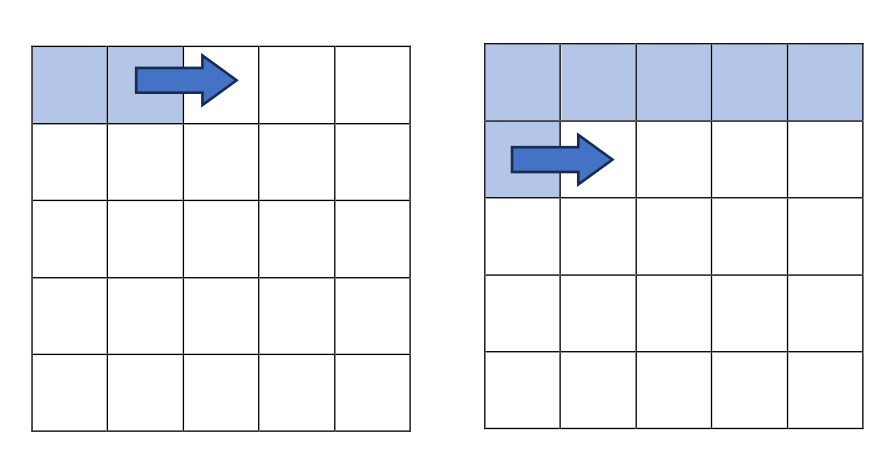
\includegraphics[width=.9\textwidth]{Assignment-1/ordered.png}
		\caption{scheme for the ordered evolution method}
		\label{fig:ordered}
	\end{figure}
\end{itemize}
After having written the program, the aim of the exercize is to perform some scalability tests on the ORFEO high-performance-computing facility. 
The scalability tests have the purpose to test and validate the code, and also test the experimental performances of the ORFEO cluster and confront 
them to the expected ones. The scalability tests that I have performed, as required for the assignment, are the following:
\begin{itemize}
	\item \textbf{Strong MPI scalability:} given a fixed size of the matrix representing the game playground,
	show the run-time behaviour increasing the number of MPI tasks (using as many nodes as possible, depending on the machine). This can be done for 
	several sizes of the playground matrix
	\item \textbf{Weak MPI scalability:} given a fixed number of MPI processes, show the run-time behaviour keeping the workload 
	each of them has to do constant. 
	\item \textbf{openMP scalability:} fix the number of MPI tasks to 1 per socket, and report the behaviour of the code increasing the number of
	threads per task from 1 up to the number of cores present on the socket.
\end{itemize}

\section{Methodology}\label{Methodology}

The program is written in the C programming language with the MPI and OpenMP libraries, and implements all the evolution methods described above.
The code is compiled with the gcc compiler from gnu and the mpicc wrapper from the MPI library. 
The world must be read from a pgm image file, which contains the initial configuration of the playground, and converted in an array of $k\times k$
unsigned char elements, where $k$ is the number of cells in a row or column. The choice of using an array of unsigned char is to reduce the RAM usage,
and the choice of using an array of one dimension to represent a square matrix is for letting the data be more contiguous in the memory. 
The array implements the square matrix of the Game of Life indexing the cells $(i,j)$ in the following way: array$[k*i+j]$, where $k$ is the 
side dimension fo the playground (i.e the number of rows or columns).
Inside the program the alive cells are represented with the number 255, whereas the dead ones are represented with the number 0, that are respectively
the numbers for the white and black colors in the pgm format. Moreover, to run the program, the following flags have been used:

\begin{itemize}
	\item \textbf{-i}: This flag starts the initialization routine. The program will generate a matrix of $k\times k$ random elements, that will be saved into a pgm file. The size $k$ of the matrix can be set with the flag \emph{-k}, and the filename in which the matrix is saved with the flag \emph{-f}.
	\item \textbf{-r}: This flag starts the routine which runs the game of life, in one of the evolution methods described before. 
	In this case the program will load the initial configuration (generated with the previous flag) from a file and will run the game of life
	for -n iterations (no default value), saving the intermediate configurations every -s iterations (default value is 0) where
	0 means that the intermediate configurations are not saved. This intermediate file are saved in the snapshot directory.
	\item \textbf{-e}: This flag is used to set the evolution method: 0 for the ordered evolution method; 1 for the static evolution method (default value 0)
\end{itemize}
For the scalability tests required for this assignment, the program has been run on the thin nodes (THIN partition) and also on the epyc nodes (EPYC partition),
using some bash script saved in the directory `scalability-scripts-for-SLURM`. In these files all the instruction for the resources management system have been implemented to allocate 
the resources, load the appropriate modules, and run the program. In order to have more reliable results, I measured each configuration attemped 5 times and I took the average of the results.


\section{Implementation}\label{Implementation}

In this section all the technical details about the program will be discussed, focusing in particular on the parallel implementation and the 
code optimization. The program is organized mainly in three groups of modules, follwing the ways in which the code can be run, described in the section before.

\subsection{\emph{main.c} and accessories modules:}
The \emph{main.c} module constains the \emph{main()} function of the program, whose purpose is to parse the command line arguments (the values given to 
the program through the flags) and to call the appropriate functions to run the program in the way the user decides (the initialization mode, with the flag -i 
or the run mode, with the flag -r). The function also initializes some default values. The \emph{read\_write\_pgm\_image.c} contains all the accessory functions
to manage the \emph{.pgm} image files, used to store the array of unsigned chars that represents the playground matrix. In particular, the function
\emph{read\_pgm\_image()} is used to read a \emph{.pgm} file, in which is stored an initial configuration of the playground to run, and to initialize
the array of unsigned chars, which is passed to the function through its pointer. The function \emph{write\_pgm\_image()} is used, instead, to write the array 
of unsigned chars (which represents the whole playground or a chunck of it) into a file in the \emph{pgm} format.

\subsection{initialization module:}
This module contains all the functions responsible for the initialization of a playground configuration. This module is called when the program is run with 
the -i flag, as described above.

The function \emph{initialize\_playground()} is the principal function of the module. It is convenient, for memory management reasons, to divide 
the case in which the playground is initialized without MPI (so with only a single independent process) from the case in which MPI is used to initialize the 
playground in parallel. The following function, though, calls the appropriate function to initialize the playground in serial (from the point of view
of MPI) or in parallel. The input parameters are the following:
\begin{itemize}
	\item filename: name of the file which will contain the initialized playground (\emph{pgm} format)
	\item $k$: size of the squre matrix that's going to rapresent the playground
\end{itemize}

The function \emph{initialize()} is called when the initialization is done with only one process, so serially from the point of view of MPI. 
In this case an unsigned char array of size $k\times k$ is dynamically allocated on the heap, in order to store the values of the playground. Then, 
the master thread spawns a certain number of parallel opemMP threads (the number of openMP threads can be selected outside the code exporting the environmental
variable \emph{OMP\_NUM\_THREADS}) in order to parallelize the for loop, which does the actual initialization of the values of the playground. The scheduling type
choosen in this case for the openMP threads is the static one, since each thread has to do approximately the same amount of work. The initialization is done 
calling the \emph{rand()} function, so the playground is initialized with random values, with a probability for a cell to be initially alive of $15\%$. Finally, 
the initial configuration is saved into a file with the \emph{pgm} format, using the \emph{write\_pgm\_image()} function discussed before. The filename of the
file can be selected running the program with the -f flag, otherwise the default name is \emph{initial\_configuration.pgm}. 
The function \emph{initialize\_MPI()} is called when the number of MPI processes is grater then one, so the initialization is done in parallel. The initialization procedure
is the same as the previous case, but now the workload is divided among the MPI processes. The workload division can be done in two different ways (implemented 
inside the function). The first way is to divide the whole playground array into $n$ chunks, where $n=\#MPI\_processes$ is the number of MPI processes. 
If the number of cells is not divisible by $n$, an extra cell is given to each process from the first to the k\%n-th. In this way the size of each chunk 
of the playground is given by the following formula:
\begin{equation}
	\text{size of $i$-th chunk}	= 
		\begin{cases}
			\lfloor{\frac{k*k}{n}}\rfloor + 1 \quad \text{if} \ \ k*k \pmod{n} \geq 0 \\
			\lfloor{\frac{k*k}{n}}\rfloor \quad \text{otherwise}
		\end{cases}
\end{equation}
where $n$ is the number of MPI processes, and $k$ is the edge size of the matrix playground ($k*k$ is the array size). 
The other way to distribute the worload among the MPI processes is that, if the number of cells is not divisible by $n$, the master
process takes care of the remaining cells. Also in the parallel version, each MPI process spawns a certain number of openMP threads
in order to parallelize the \emph{for} loop, in which the same computation as before is done. 
Since the main focus of this assignment is to test the scalability of the parallel code in several ways, so on the running mode, in this case 
the code was not tested in order to choose the optimal way to parallelize the initialization of the playground. 

\subsection{running modules:}
This module contains all the functions responsible for the running of a playground configuration. This module is called when the program is run with 
the -r flag, as described above. 
The function \emph{evolve\_cell()} applies the rules of the game: given a certain cell $i$, it calculates the number of alive neighbours (considering the 
periodic boundary conditions in the matrix representation of the playground array), and sets the next state of a cell (alive if the number of alive neighbours
is two or three). 
The function \emph{play\_game()} initializes MPI (in multiple mode) and checks the type of evolution selected by the user (-e flag), calling the correct function to play the game of life on the playground.
In particular, for $e=0$ it calls the ordered evolution function, and for $e=1$ the static evolution function. Then it measures the execution time for each of 
the evolution modes. The input arguments are the following:
\begin{itemize}
	\item filename: name of the file containing the initial configuration of the playground
	\item $k$: size of the squre matrix that rapresents the playground
	\item $n$: number of generations for which the game of life will run
	\item s: frequency for saving a snapshot of the playground
	\item e: flag for the evolution mode: 0 -> ordered evolution, 1 -> static evolution
\end{itemize}
Then there are the two core functions of the program, which perform the actual evolution of the playground.
\subsubsection{The ordered evolution method}
Since in the ordered method the evaluation of the next state of the $n$-th cell depends on the result of the evaluation of the previous one, 
the task is intrinsically serial, and the domain decomposition approach will not improve the execution time. For this reason the ordered evolution 
is executed with a single MPI task. This function works in this way:
\begin{enumerate}
	\item the function allocates on the heap (using the \emph{malloc()} method) enough memory to store the initial configuration of the playground, 
	so it allocates an array of size $k\times k$. Then the array is initialized with the \emph{read\_pgm\_image()} function which reads from a file 
	the initial configuration of the playground and fills the array values. 
	\item evaluates the next state of cell $i$ with the \emph{evolve\_cell()} function and update immediately the result by overwriting the previous value
	in the array that represents the current state of the playground. In fact, in the ordered evolution of the playground the next state of a cell 
	is computed and updated before moving to the next cell.
	\item eventually saves a snapshot of the playground (in the directory \emph{snapshots}) according to the value given by the user to the flag -s 
	(which specifies the saving frequency). 
	\item it repets the steps 2 and 3 for $n$ times, where $n$ is the number of evolutions to be computed, which is selected by the user with the -n flag.
	\item finally it saves the final state of the playground into a pgm file. 
\end{enumerate}
In this evolution method, the parallelization is done only using OpenMP. In particular, the inner \emph{for} loop (the one which does the actual computation)
is parallelized with the \emph{\#pragma omp parallel for} directive.
\subsubsection{The static evolution method}
In this type of evolution, the playgroud is "freezed" and there is a disentanglement between the status evaluation of a cell, and the status update in the 
playground array. So, the function has to evaluate the next status of each cell (until the last one) and memorize it (in a temporary array), 
and only then update all the playground array. This means that it is possible to use the domain decomposition approach to parallelize the program with MPI,
giving to each process a chunk of the playground array to evaluate. This is, though, the most interesting part.
The function \emph{static\_evolution()} performs the static evolution of the playground and saves the final state of the playground (and eventually some intermediate snapshots) into a pgm file. 
It is convenient to divide the case in which there is only one MPI process (in this case the evolution is serial of course) from the case in which 
there are multiple independent MPI processes performing the static evolution in parallel.
For this purpose, the function checks if the number of MPI processes (the size of the world communicator) is grater than one, 
and calls the appropriate function in which the actual computation is done. The input arguments are the following:
\begin{itemize}
	\item filename: name of the file containing the initial state of the playground
	\item $k$: size of the squre matrix that rapresents the playground
	\item $n$: number of generations for which the game of life will run
	\item s: snapshot saving frequency
	\item rank: rank of the MPI process
	\item size: number of MPI processes
\end{itemize}
The function \emph{serial\_static()} is called only if the program is executed on a single process, and performs the static evolution is serial, 
saving the final configuration into a pgm file. The static serial implementation follows a procedure that is quite similar to the ordered method, 
with the difference that the new evaluated state of a cell is not immediately updated in the whole playground, but saved in a temporary array. The 
actual update is done at the end. For this reason, the static evolution needs exactly the double of the space with respect to the ordered method, 
since it needs to store the current state of each cell and the new evolved one in two different arrays, since the update of the playground
is done only at the end of the computation of each cell's new state. The threadization with openMP is done within the single MPI process used. 
The function \emph{parallel\_static()} is called only if the program is executed on more than one process, and performs the static evolution of the playground 
in parallel with multiple MPI processes. In this case workload is splitted among the MPI processes, and the whole playground is divided in $n$ chunks,
where $n$ is the number of MPI processes. In particular, the $i$-th process is associted to a chunk of size given by the equation:
\begin{equation}
	\text{size of $i$-th chunk}	= 
		\begin{cases}
			\lfloor{\frac{k*k}{n}}\rfloor + 1 \quad \text{if} \ \ k*k \pmod{n} \geq 0 \\
			\lfloor{\frac{k*k}{n}}\rfloor \quad \text{otherwise}
		\end{cases}
\end{equation}
The parallel function works in this way:
\begin{enumerate}
	\item each MPI process autonomously allocates on the heap (using the \emph{malloc()} method) enough memory to store the initial configuration of the playground, 
	(array of size $k\times k$). Then the array is initialized by each MPI process with the \emph{read\_pgm\_image()} function which reads from a file 
	the initial configuration of the playground and fills the array values. In this way all the MPI processes have always a copy
    of the whole playground of the game, and there is no need of MPI communications among them to exchange
    the boundary values, needed for the computation of a cell's next state. 
    This choice has the advantage to reduce the MPI communications among the processes (this can lead to 
    less computational time) but is more expensive for the point of view of the memory. In fact, each process has to 
    allocate memory for storing the state of cells that it is not going to use. This can be a problem if the dimension of the grid is very large.
	\item every MPI process computes some needed variables to distribute the computational work among them.
	\begin{itemize}
		\item lenghts: an array containing the dimension of the chunk associated to each independent MPI process
		\item displacements: an array containing the displacements (the position) of the chunk in the global playground array, for each process
	\end{itemize}
	These variables are needed for the MPI function \emph{MPI\_Allgatherv()} used later. The computation of these variables introduce a little time overhead. 
	\item Each MPI process allocates an additional array needed to store temporarlly the new states of each cell, before doing the whole upgrade of the actual playground.
	\item Each MPI process evaluates (in parallel) the next state of the cells in its chunk, with the function \emph{evolve\_cell()}, and stores
	the result in the additional array. In doing this, each MPI process can spawn a certain number of openMP threads, in order to add a new level of parallelism.
	Then every process send its chunk to all the others (with the \emph{MPI\_Allgatherv} function). This is needed because in the next iterations each
	MPI process will need to have a copy of the whole playground array.
	\item eventually the master process (the one with rank $= 0$) saves a snapshot of the playground (in the directory \emph{snapshots}),
	according to the value given by the user to the flag -s (which specifies the saving frequency).
	\item each process repets the previous step for $n$ times, where $n$ is the number of evolutions to be computed, 
	waiting for all the processes to finish the computation of the previous iteration (using the \emph{MPI\_Barrier} function).
	\item finally the master process saves the final state of the playground into a pgm file.
\end{enumerate}


\section{scalability results}\label{Results}
In the following section the results of the scalability tests, described in the previous section, will be presented. 
For each configuration of flags tested, the program was run 5 times and then the average time was computed. 
Moreover, in order to have more reliable results, it was requested to SLURM the exclusive usage of the
whole node (or nodes) in which the code had to run. In order to have a higher optimization effect, each program was compiled (with the command \emph{make}
using the \emph{Makefile}) in a node with the same architecture of the node the program was run on (this is important for the compiling directive 
\emph{--march=native}). As specified before, the program was tested both on the EPYC nodes and on the THIN ones. 

\subsection{openMP scalability}
For this scalability test it was requested to fix the number of MPI tasks to 1 per socket, and report the behaviour of the code increasing 
the number of threads per task from 1 up to the number of cores present on the socket. The openMP scalability test was done, in this work, using both 1
and 2 sockets (so 1 and 2 MPI processes per socket respectively), always on the same node. In particular, the EPYC nodes are equiped with two 64-cores sokets per machine (for a total number of 128 cores per machine),
and the THIN nodes are equiped with two 12-core sokets per machine (for a total number of 24 cores per machine). In order to reach this result, 
the openMP environment variables were set as \emph{export OMP\_PLACES=cores} and \emph{export OMP\_PROC\_BIND=close} in each configuration. Moreover, since for 
these tests was used a single node at a time, to place the MPI processes on the sokets, the option \emph{--map-by socket} of \emph{mpirun} was used. 
To do that, we can also use the environment variable \emph{export I\_MPI\_PIN\_DOMAIN=socket}. To perform this scalability test, two different sizes of the square playground
have been used: $10000^2$ and $17500^2$. Moreover, after having measurd the time execution of the code for each configuration, the speedup $Sp$ and the efficiency $Eff$ of the code
have been computed, with the following formulas:
\begin{equation}
	Sp(p,k) = \frac{T_s(k)}{T_p(k)} \ ,
\end{equation}
\begin{equation}
	Eff(p,k) = \frac{Sp(p,k)}{p} \ ,
\end{equation}
where $T_s(k)$ is the time taken by the serial version of the code to solve a problem of size $k$, and
$T_p(k)$ is the time taken by the parallel version of the code to solve a problem of size $n$, with $p$ computing units.
Ideally, to reach the perfect scalability, the code should have a speedup that is perfectly linear with the number of threads used and an efficiency that is equal to 1. 
So it is auspicable, for a good code, to have a speedup that is closely linear, and an efficiency that is not too far from 1.
Below are reported all the graphs for the openMP scalability, realized running the program in the static evolution way.
For the THIN nodes we have the following graphs for time scalability, speedup and efficiency (for different sizes of the playground): \\
\begin{figure}[H]
	\centering
	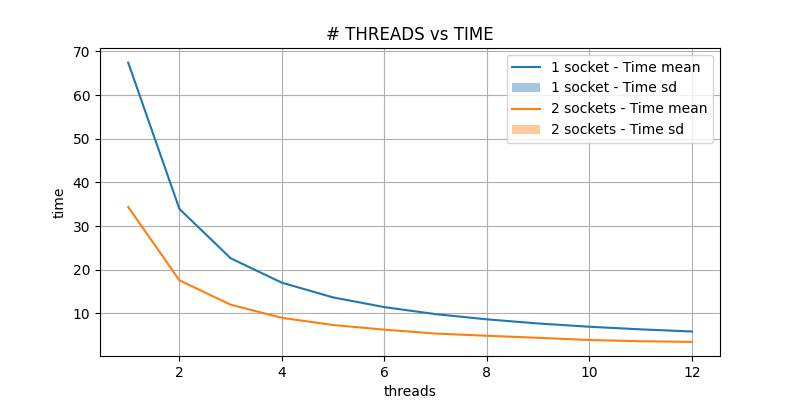
\includegraphics[width=\textwidth]{Assignment-1/OMP-static-10000-10-THIN-1sockettime.png}
	\caption{time scalability for a playground of size $10000^2$ on THIN node}
\end{figure}
\begin{figure}[H]
	\centering
	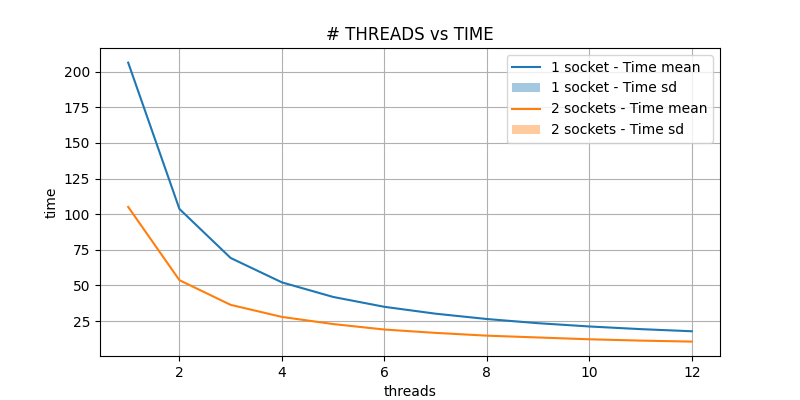
\includegraphics[width=\textwidth]{Assignment-1/OMP-static-17500-10-THIN-1sockettime.png}
	\caption{time scalability for a playground of size $17500^2$ on THIN node}
\end{figure}
\begin{figure}[H]
	\centering
	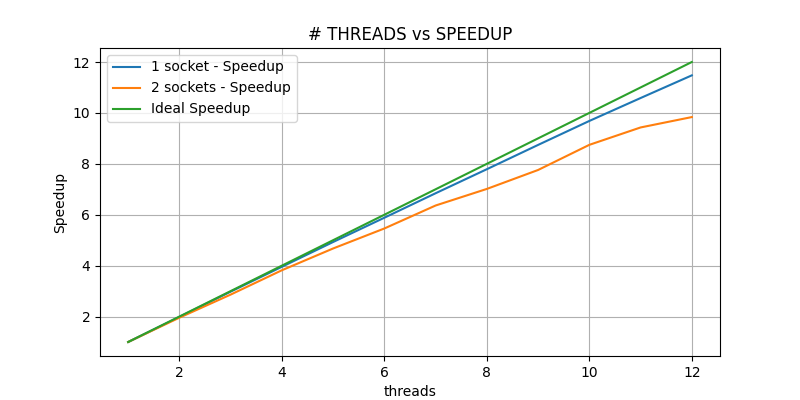
\includegraphics[width=\textwidth]{Assignment-1/OMP-static-10000-10-THIN-1socketspeedUp.png}
	\caption{speedup for a playground of size $10000^2$ on THIN node}
\end{figure}
\begin{figure}[H]
	\centering
	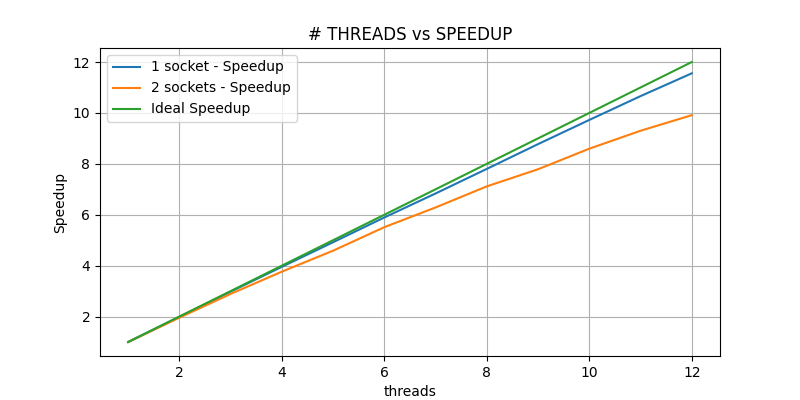
\includegraphics[width=\textwidth]{Assignment-1/OMP-static-17500-10-THIN-1socketspeedUp.png}
	\caption{speedup for a playground of size $17500^2$ on THIN node}
\end{figure}
\begin{figure}[H]
	\centering
	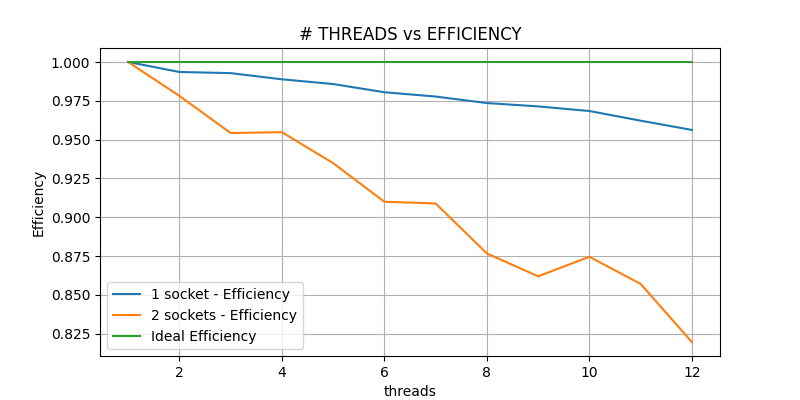
\includegraphics[width=\textwidth]{Assignment-1/OMP-static-10000-10-THIN-1socketefficiency.png}
	\caption{efficiency for a playground of size $10000^2$ on THIN node}
\end{figure}
\begin{figure}[H]
	\centering
	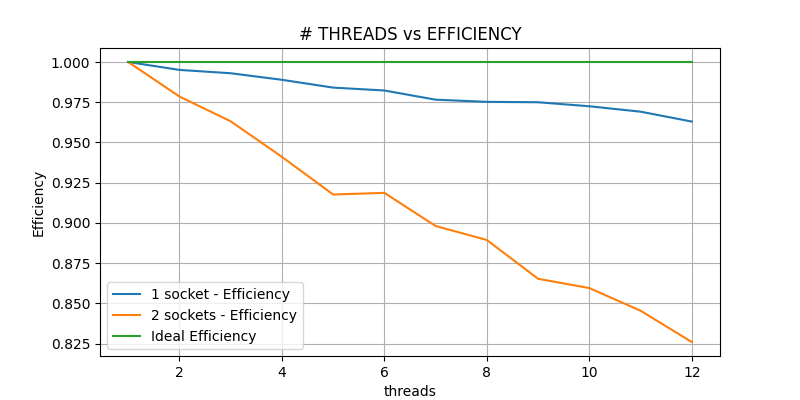
\includegraphics[width=\textwidth]{Assignment-1/OMP-static-17500-10-THIN-1socketefficiency.png}
	\caption{efficiency for a playground of size $17500^2$ on THIN node}
\end{figure}
For the EPYC nodes we have the following graphs for time scalability, speedup and efficiency (for different sizes of the playground):
\begin{figure}[H]
	\centering
	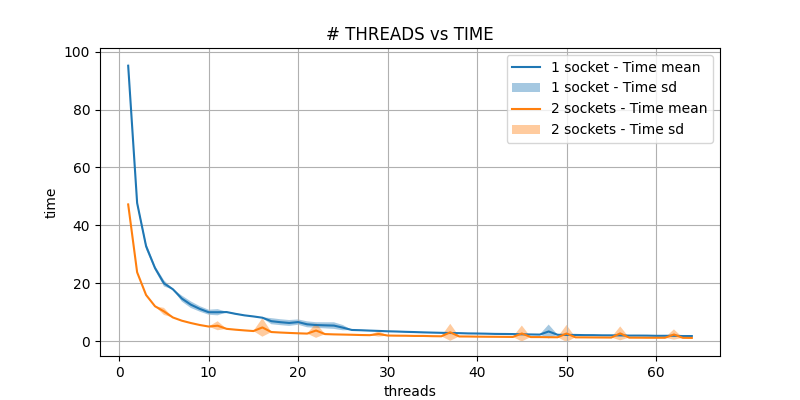
\includegraphics[width=\textwidth]{Assignment-1/OMP-static-10000-10-EPYC-1sockettime.png}
	\caption{time scalability for a playground of size $10000^2$ on EPYC node}
\end{figure}
\begin{figure}[H]
	\centering
	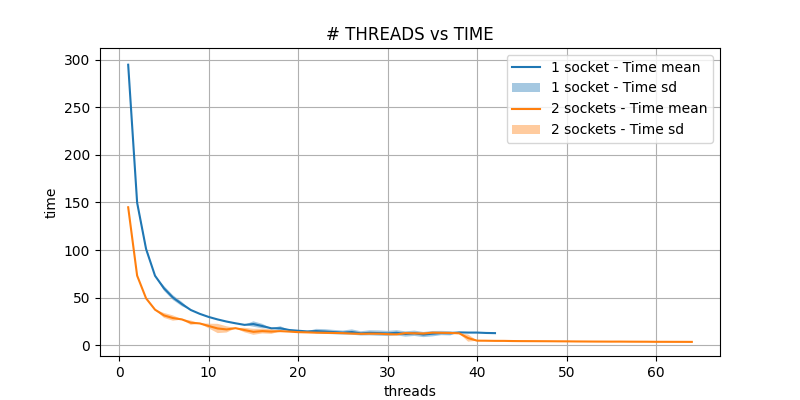
\includegraphics[width=\textwidth]{Assignment-1/OMP-static-17500-10-EPYC-1sockettime.png}
	\caption{time scalability for a playground of size $17500^2$ on EPYC node}
\end{figure}
\begin{figure}[H]
	\centering
	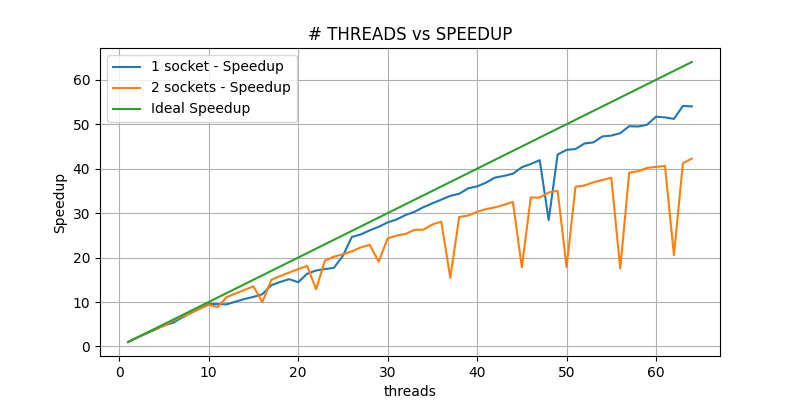
\includegraphics[width=\textwidth]{Assignment-1/OMP-static-10000-10-EPYC-1socketspeedUp.png}
	\caption{speedup for a playground of size $10000^2$ on EPYC node}
\end{figure}
\begin{figure}[H]
	\centering
	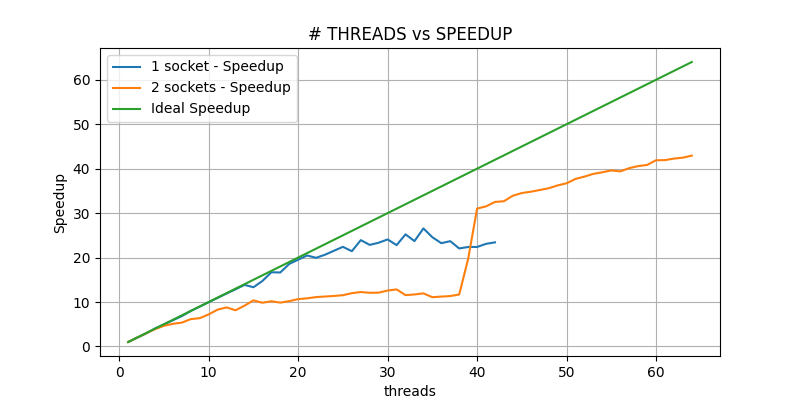
\includegraphics[width=\textwidth]{Assignment-1/OMP-static-17500-10-EPYC-1socketspeedUp.png}
	\caption{speedup for a playground of size $17500^2$ on EPYC node}
\end{figure}
\begin{figure}[H]
	\centering
	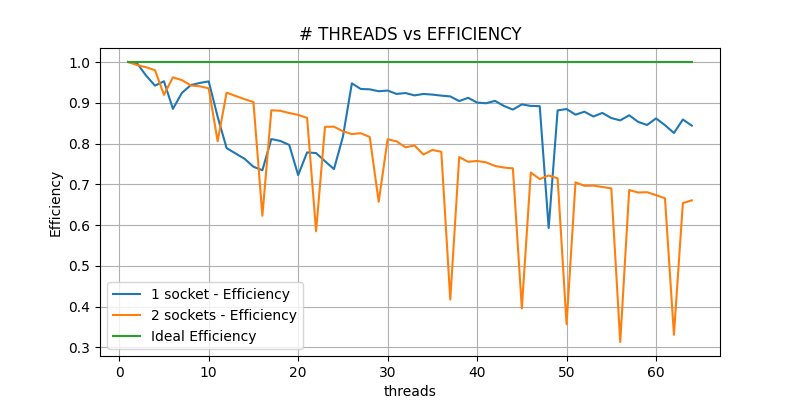
\includegraphics[width=\textwidth]{Assignment-1/OMP-static-10000-10-EPYC-1socketefficiency.png}
	\caption{efficiency for a playground of size $10000^2$ on EPYC node}
\end{figure}
Analyzing these plots we can state some conclusions:
\begin{itemize}
	\item The code scales with with respect to the number of OpenMP threads
	\item The scalability tests conducted on the THIN nodes have always an efficiency greater than $80\%$, which is very satisfying
	\item The scalability tests conducted on the THIN nodes have always a speedup that is closer to the linear growth
	\item These scalability tests have underlined a different behaviour on the EPYC nodes. In fact, the global profile of each curve is similar to the 
	one obtained on the THIN nodes, but, for some values of openMP threads, there are lacks of seedup and efficiency. This fact gives to the curves obtained
	on the EPYC nodes a whole jagged profile. 
\end{itemize}
For the ordered evolution method, the program is strictly serial, and then the elapsed time is constant, or, in the worst case, it increases due 
to the parallelization overhead. 


\subsection{Strong MPI scalability}
The aim of this scalability test is to show the run-time behaviour of the code, increasing the number of MPI tasks, maintaining a fixed size of the matrix 
representing the game playground. For this scalability test, 2 EPYC nodes and 2 THIN nodes have been used. As specified before, the EPYC nodes are equiped with two 64-cores sokets per machine 
(for a total number of 256 cores for two machines), and the THIN nodes are equiped with two 12-core sokets per machine (for a total number of 48 cores in total for two nodes).
Since we are interested in the MPI scalability, the following openMP environment variables have been set: \emph{export OMP\_PLACES=cores}, 
\emph{export OMP\_PROC\_BIND=close}, and \emph{export OMP\_NUM\_THREADS=1} in order to fix the openMP threads for each task to be 1.
For the placement of the MPI processes, the \emph{--map-by core} option of \emph{mpirun} has been used, leaving the default \emph{--bind-to socket}.
Of course, this scalability test can be performed only for the static evolution method, since the ordered evolution method is serial from the point of 
view of MPI. For the tests run on the THIN nodes, three configurations have been used:
\begin{itemize}
	\item $k\times k = 10000^2$ and $n=10$ generations
	\item $k\times k = 12500^2$ and $n=10$ generations
	\item $k\times k = 17500^2$ and $n=10$ generations
\end{itemize}
Below are reported the graphs for the static evolution method.
\begin{figure}[H]
	\centering
	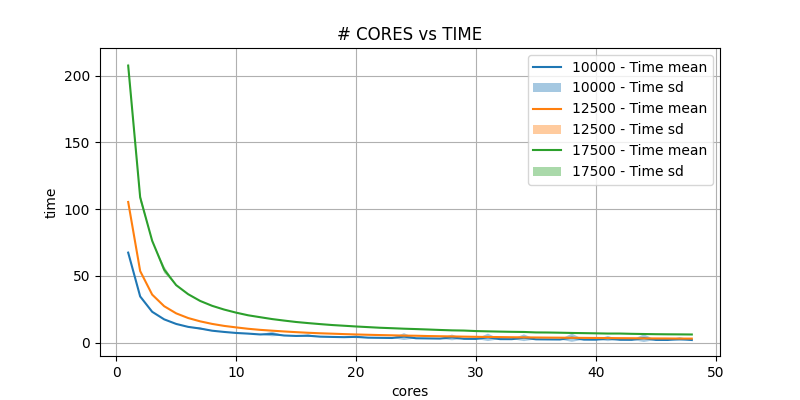
\includegraphics[width=\textwidth]{Assignment-1/MPI_strong-static-10000-10-THINtime.png}
	\caption{time scalability for strong MPI tests: the graph plots the number of MPI processes (so the number of core used) versus the time 
	of execution of the code}
\end{figure}
\begin{figure}[H]
	\centering
	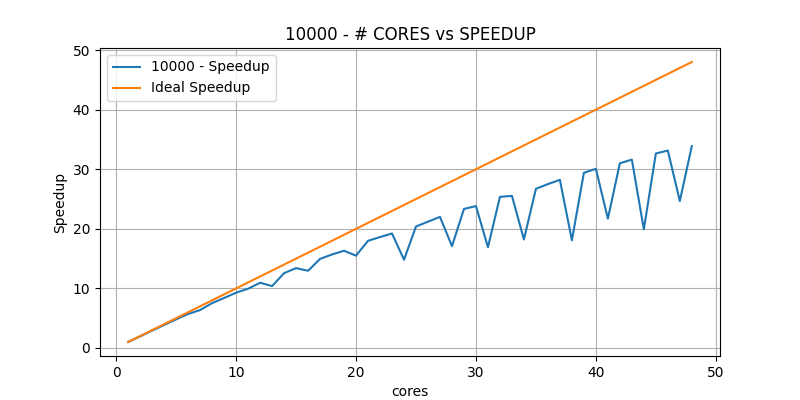
\includegraphics[width=\textwidth]{Assignment-1/MPI_strong-static-10000-10-THIN10000_speedUp.png}
	\caption{Speedup with size $k=10000$}
\end{figure}
\begin{figure}[H]
	\centering
	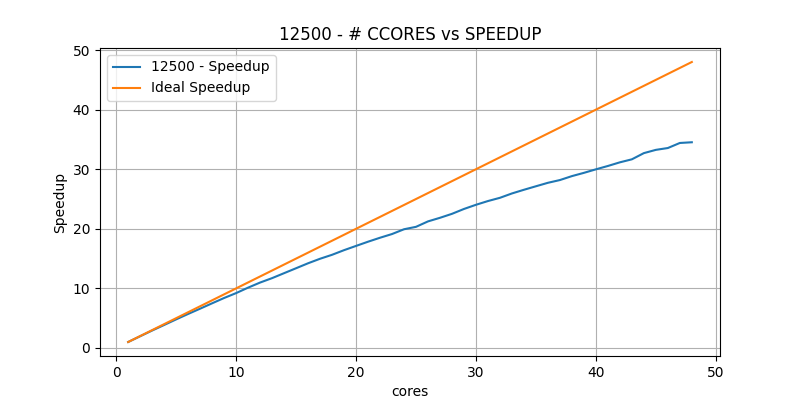
\includegraphics[width=\textwidth]{Assignment-1/MPI_strong-static-12500-10-THIN12500_speedUp.png}
	\caption{Speedup with size $k=12500$}
\end{figure}
\begin{figure}[H]
	\centering
	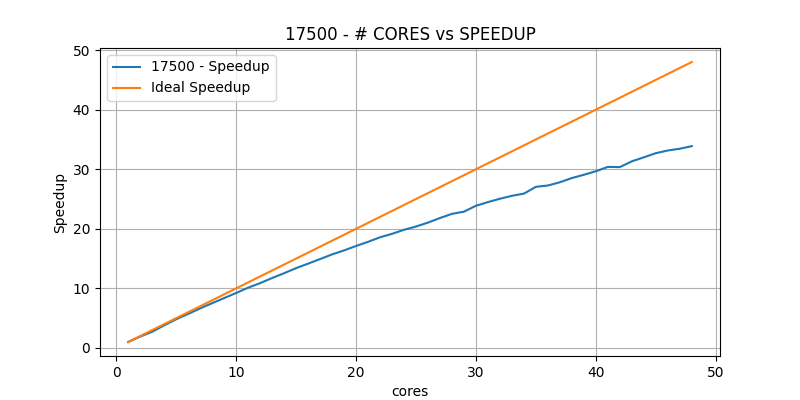
\includegraphics[width=\textwidth]{Assignment-1/MPI_strong-static-17500-10-THIN17500_speedUp.png}
	\caption{Speedup with size $k=17500$}
\end{figure}
\begin{figure}[H]
	\centering
	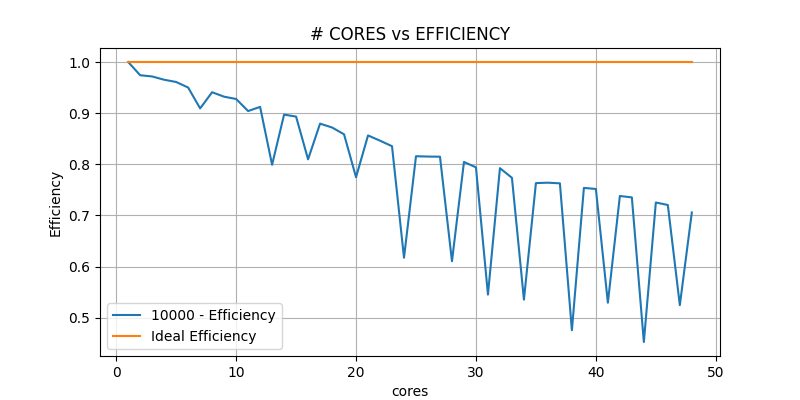
\includegraphics[width=\textwidth]{Assignment-1/MPI_strong-static-10000-10-THIN10000_efficiency.png}
	\caption{efficiency with size $k=10000$}
\end{figure}
\begin{figure}[H]
	\centering
	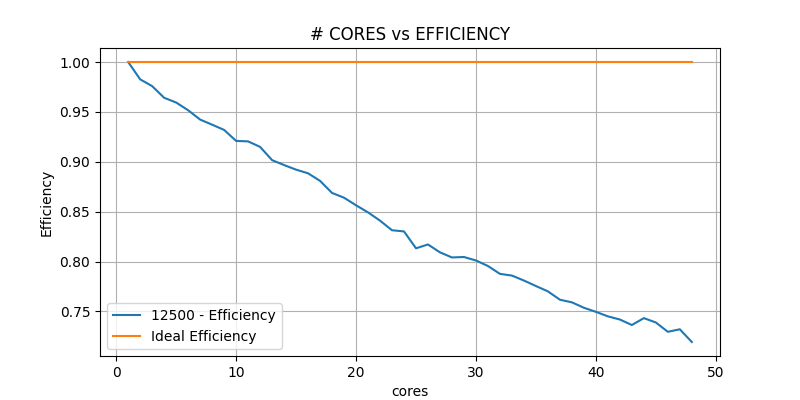
\includegraphics[width=\textwidth]{Assignment-1/MPI_strong-static-12500-10-THIN12500_efficiency.png}
	\caption{efficiency with size $k=12500$}
\end{figure}
\begin{figure}[H]
	\centering
	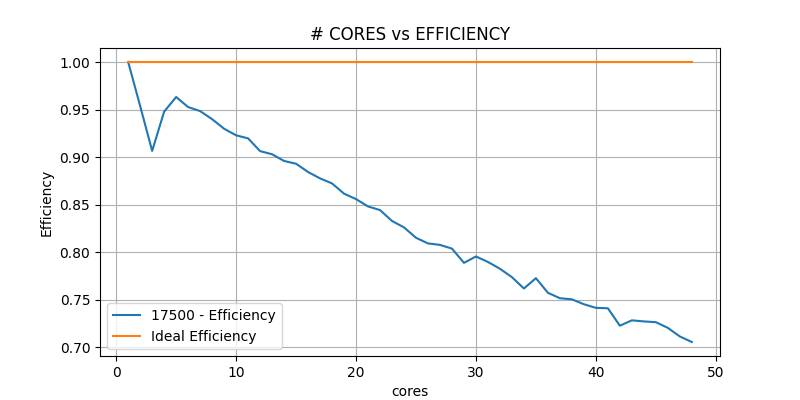
\includegraphics[width=\textwidth]{Assignment-1/MPI_strong-static-17500-10-THIN17500_efficiency.png}
	\caption{efficiency with size $k=17500$}
\end{figure}
For the tests run on the EPYC nodes, the following configurations have been used:
\begin{itemize}
	\item $k\times k = 10000^2$ and $n=10$ generations
	\item $k\times k = 12500^2$ and $n=10$ generations
	\item $k\times k = 12500^2$ and $n=25$ generations
	\item $k\times k = 17500^2$ and $n=10$ generations
\end{itemize}
Only in this case, for the EPYC nodes, these configurations have been run once, not 5 times. This choice is due to time management reasons, 
since EPYC nodes have 128 cores per machine (against the 24 of THIN machines), and to perform a complete scalability test over all the cores is quite time expensive.
\begin{figure}[H]
	\centering
	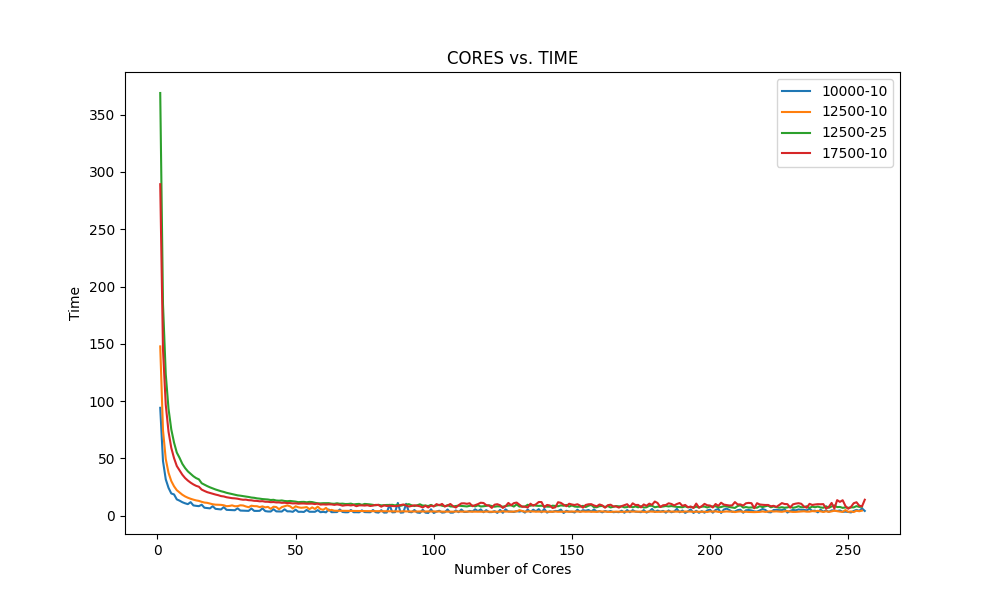
\includegraphics[width=\textwidth]{Assignment-1/cores_vs_time.png}
	\caption{strong MPI time scalability, on EPYC nodes}
\end{figure}
\begin{figure}[H]
	\centering
	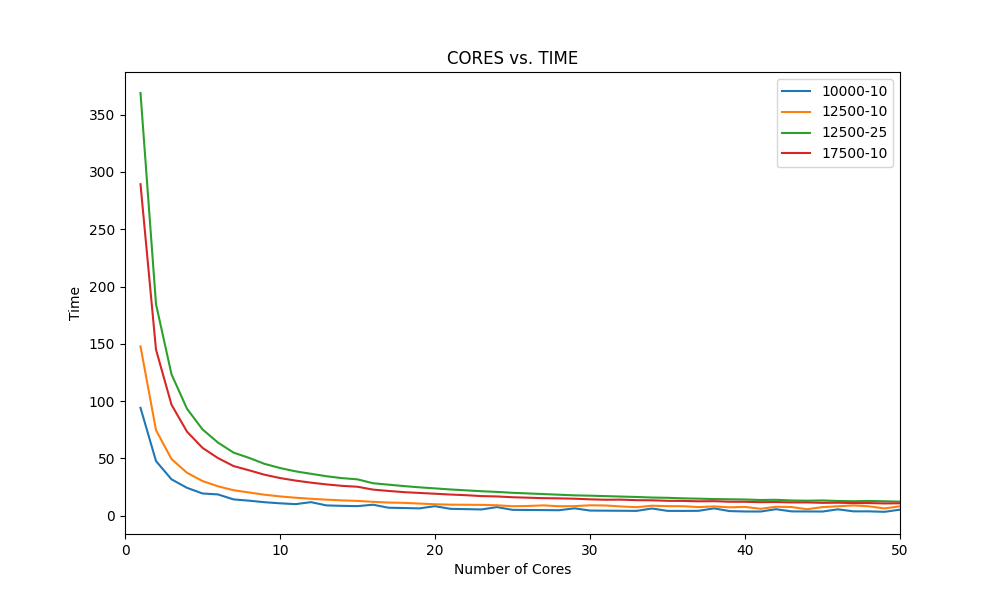
\includegraphics[width=\textwidth]{Assignment-1/cores_vs_time_focus.png}
	\caption{strong MPI time scalability, on EPYC nodes. Focus on the range of cores [0-50]}
\end{figure}
\begin{figure}[H]
	\centering
	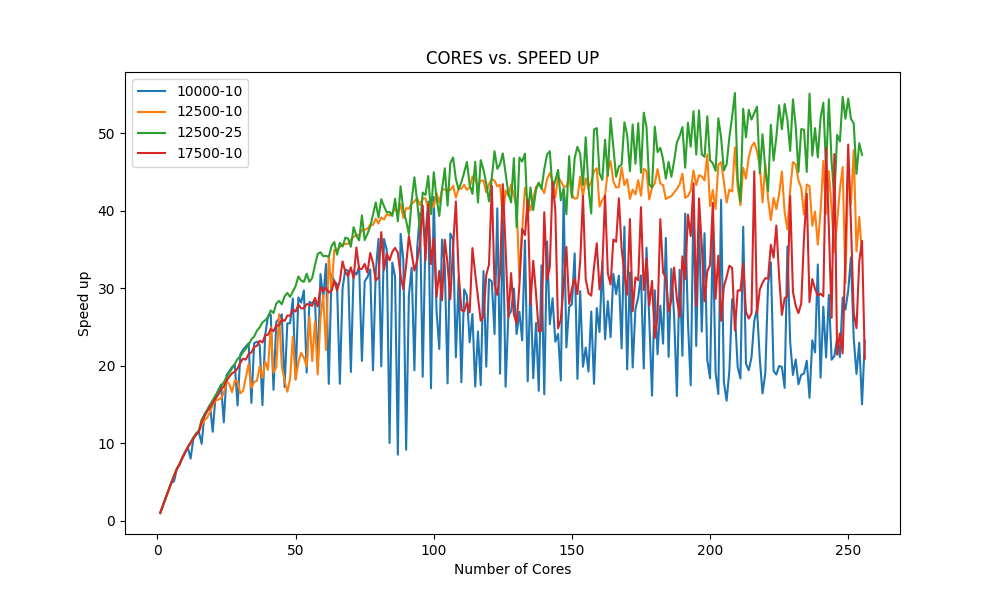
\includegraphics[width=\textwidth]{Assignment-1/cores_vs_speedUp_2.png}
	\caption{Speedup}
\end{figure}
\begin{figure}[H]
	\centering
	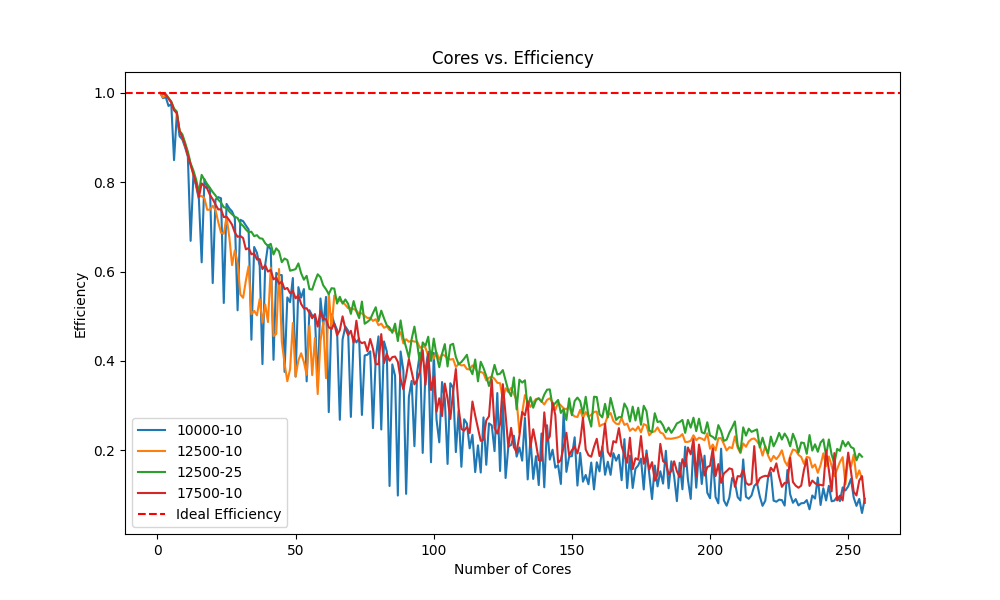
\includegraphics[width=\textwidth]{Assignment-1/cores_vs_efficiency_2.png}
	\caption{efficiency}
\end{figure}


Analyzing these plots we can state some conclusions:
\begin{itemize}
	\item The strong MPI scalability is quite satisfying in particular on the THIN nodes, as the speedup still increases
	with the number of MPI processes, and is close to the linear behaviour (of course not perfectly linear). The scalability tests on the EPYC nodes
	have worsen results, since the speedup looses the linear trend evidently after 20 MPI processes used, and tends to a flat behaviour as the number of 
	MPI processes grows.
	\item The efficiency have a similar behaviour with respect to the speedup discussed before. For the tests run on the THIN nodes, 
	it decreases with an acceptable rate: up to 48 MPI processes, the efficiency is still above the 70\%, for each size configuration (except for $10000^2$).
	The configuration with size $10000^2$ has reported a jagged profile, differently from the other sizes. The tests on the EPYC nodes report worsen results:
	the efficiency drops evidently under the value of 1 after 20 MPI processes, and tends to 0 as the number of MPI processes increases.
	Up to 256 MPI processes, the efficiency is above the 20\%, and the lines have jagged profiles.
\end{itemize}

\subsection{Weak MPI scalability}
The aim of this scalability test is to show the run-time behaviour of the code, with a fixed number of MPI processes but keeping the workload of each
MPI process constant. In the program, the workload is represented by the size of the playground, which is a square grid of size $k\times k$, implemented 
with an array of lenght $K*k$. The parameter $k$ can be used, then, as a measure of the workload. In order to keep the workload of each
MPI process constant, the relation between the workload with $n$ MPI processes, and the number $n$ of MPI processes must be the following:
\begin{equation}
	\frac{k(n)^2}{n} = c = k(1)*k(1) \ ,
\end{equation}
where $k(n)$ is the side size of the playground (so the workload) using $n$ MPI processes, $n$ is the number of MPI processes, and c is a costant value, that is equal to the 
workload associated to 1 single MPI process. We can fix this value to $c=10000^2$. At this point, we can easly find the value $k(n)$ of the workload 
for $n$ MPI processes:
\begin{equation}
	k(n) = \sqrt{c*n} \ .
\end{equation}
Using, for example, 9 different numbers of MPI processes, the workload associated to each case is given by:
\begin{center}
	\begin{tabular}{|c c|}
	\hline 
	$n$ & $k(n)$  \\
	\hline
	1 & $10000$ \\
	2 & $14142$	\\
	3 & $17321$	\\
	4 & $20000$	\\
	5 & $22361$	\\
	6 & $24495$	\\
	7 & $26458$	\\
	8 & $28284$	\\
	9 & $30000$	\\
	\hline
	\end{tabular}
\end{center}
Finally, below are reported the graphs obtained with the weak MPI scalability tests. 
In particular, the scalability tests have been performed using both 1 and 16 OpenMP threads, expecting to see a constant execution time in both cases.
Also in this case, the tests have been performed on THIN nodes and EPYC nodes, and only for the static evolution method, since the ordered one is intrinsically
serial, and it is not implemented using MPI.
\begin{figure}[H]
	\centering
	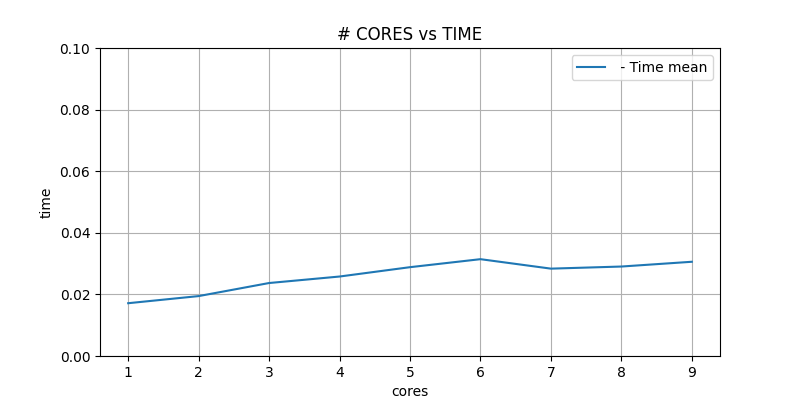
\includegraphics[width=\textwidth]{Assignment-1/MPI_W-scalability_static-ev_1omp-threds-THIN_time.png}
	\caption{weak MPI time scalability with 1 openMP thread, on THIN node}
\end{figure}
\begin{figure}[H]
	\centering
	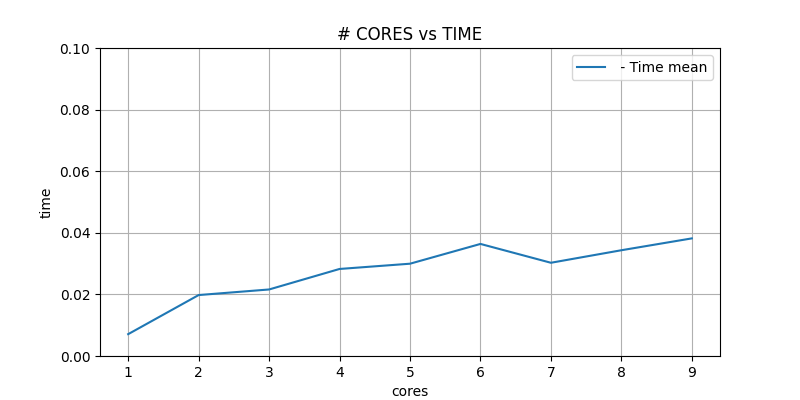
\includegraphics[width=\textwidth]{Assignment-1/MPI_W-scalability_static-ev_16omp-threds-THIN_time.png}
	\caption{weak MPI time scalability with 16 openMP thread, on THIN node}
\end{figure}
\begin{figure}[H]
	\centering
	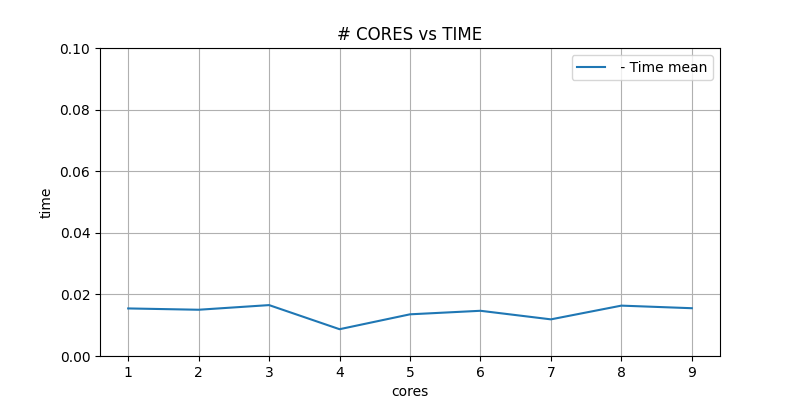
\includegraphics[width=\textwidth]{Assignment-1/MPI_W-scalability_static-ev_1omp-threds_time.png}
	\caption{weak MPI time scalability with 1 openMP thread, on EPYC node}
\end{figure}
\begin{figure}[H]
	\centering
	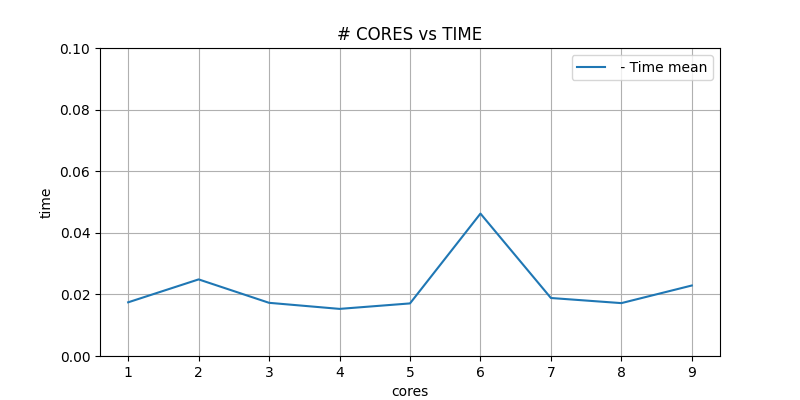
\includegraphics[width=\textwidth]{Assignment-1/MPI_W-scalability_static-ev_16omp-threds_time.png}
	\caption{weak MPI time scalability with 16 openMP thread, on EPYC node}
\end{figure}
As expected, the execution time is approximately constant because the workload for each MPI process is the same. 

\section{Final considerations}\label{Final}
In conclusion, the program implements in a satisfying way the parallel version of the Conway's game of life, providing expectable and good results
in the scalability tests performed (from the point of view of time scalability, seedup and efficiency), in particular for the THIN nodes. Some possible
improvements that can be done to enhance the performance of the code can be the following:
\begin{itemize}
	\item the functions used to read and write the \emph{pgm} images are serial. In particular, the function \emph{write\_pgm\_image()} is always called 
	by the master process. A parallel version of them can be implemented, for example using \emph{MPI-IO}.
	\item as said before, in the function \emph{parallel\_static()}, all the MPI processes have always a copy of the whole playground of the game, 
	even if they work only on a chunk of the whole playground. We can implement a different version of the function, in which each parallel MPI task
	allocates the memory that is necessary only for its chunk of the playground. This means that there is the need of communication between the MPI 
	processes in order to exchange the neighbour cell states necessary for the computation (and not present in the chunck). This procedure is not going
	to improve the execution time (probability it introduce some communication overhead) but certainly the memory management, allowing to store grater 
	playgrounds. 
\end{itemize}

%%%%%%%%%%%%%%%%%%%%%%%%%%%%%%%%%%%%%%%%%%%%%%%%%%%%%%%%%%%%%%%%%%%%%%%%%%
\chapter{Assignment 2}

\section{Overview}
% Your content for the Overview section goes here.
The exercise 2 consists in doing benchmark of 3 different libraries on the given file \textit{dgemm.c} on the supercomputer ORFEO.

The 3 libraries are \textit{mkl}, \textit{openBLAS} and \textit{blis}. The first two libraries were already loaded in ORFEO. So, we could just load them with
\begin{verbatim}
    module load mkl/latest
    module load openBLAS/0.3.23-omp
\end{verbatim}
In order to work with blis, we needed to manually download the blis folder, since we needed blis headers and libraries. 

The given file dgemm.c (General Matrix Multiplication) is a matrix multiplication benchmark. In this file, there is the multiplication between 2 matrices of respective size of $n \times k $ and $ k \times m$. In our specific case, we selected 2 square matrices of the same size, namely 
\begin{equation*}
  n = k = m .   
\end{equation*}
The needed floating point operations are $n^3$ and the memory references $4n^2$. Since the number of floating point operations has a greater order of growth with respect of the number of memory references, there is the possibility to became very efficient when the $n$ increases.

We tested two parameters: 
\begin{itemize}
    \item The \textbf{time} needed to execute the file.
    \item The \textbf{GFloaps}: a unit of measurement of the performance of processing speed of a computing system (or a single computer). Especially, one GFloaps is the number of floating point operations that a computer system is able to perform in a second. 
\end{itemize}
The floating point operations involve real numbers, so it makes sense to ask how many digits do we consider to represent them. For this reason, we divided the benchmarks in two parts: one storing numbers with single precision (float) and one with double precision (double). \
We changed the name of the original file \textit{dgemm.c} in \textit{gemm.c}, so during all the exercise the files with the prefix \textit{sgemm} are the ones that use single precision and with the prefix \textit{dgemm} the ones with double precision. 

\section{ORFEO Performance features}
Before starting we wanted to discuss two performance features proper of ORFEO:
\begin{itemize}
    \item Peak performance 
    \item Speed up factor (when cores increase)
\end{itemize}

\subsection{The peak performance}
The peak performance refers to the maximum computational processing power that a system can achieve under ideal conditions. It represents the theoretical upper bound of performance of a supercomputer. Peak performance is measured in terms of floating-point operations per second.
The peak performance is defined by
\begin{equation}
\label{pp}
PP = \text{Number of cores} \times \text{Clock Speed (in Hertz)} \times \text{FLOPC}    
\end{equation}
where FLOPC is the floating point operations per clock cycle.
As we can see n the equation \ref{pp}, the peak performance depends on the cores, so it make sense to compute the ORFEO peak performance when we fix the number of used cores.
Moreover, machine precision can significantly impact the calculation and representation of FLOPC.
Since the ORFEO clock speed is 2.6 GHz and since the nodes can manage 32 single precision floating point operations per cycle and 16 double precision floating point operations per cycle,
\begin{align}
\text{PP}_{Epyc,float} =   64 * 2.6 \text{ GHz } * 32 \text{ FLOPC }  = 5324.8 \text{ GFLOPS}\\
\text{PP}_{Epyc,double} =  64 * 2.6 \text{ GHz } * 16 \text{ FLOPC }  = 2662.4 \text{ GFLOPS}
\end{align}
As reported in the slides, the 10 THIN nodes have a peak performance of 1997 GFLOPS then 12 cores has a peak performance of 2396 GFLOPS for single precision, while for double precision 1198 GFLOPS.

\subsection{Speed up}
While we discussed the peak performance for the first point of the exercise (scaling on size), for the second point (strong scalability) we are interested in the speed up function. 
The speed up function take in input the size of the problem and the number of processors we use and returns the speed up we get using $p$ processors instead of 1. Formally,
\begin{equation}
    \text{Speed up = } \text{Sp}(n,p) = \frac{T_s(n)}{T_p(n)}
\end{equation}
where $T_s(n)$ is the time needed to execute a problem of size n in serial and $T_p(n)$ is the time needed if you solve it in parallel with $p$ processors.


\section{Steps Done}
% Your content for the Steps Done section goes here.
\subsection{Preliminary work: the makefile}
As we wrote in the overview section, we first thing we did was change the name of the \textit{dgemm.c} file in \textit{gemm.c} to avoid confusion.

The second step was doing a proper modification to the makefile in order to be able to "make" 5 executable:
\begin{itemize}
    \item sgemm mkl.x: gemm file with single precision compiled with mkl library 
    \item dgemm mkl.x: gemm file with double precision compiled with mkl library
    \item sgemm oblas.x: gemm file with single precision compiled with oblas library
    \item dgemm oblas.x: gemm file with double precision compiled with oblas library
    \item sgemm blis.x: gemm file with single precision compiled with blis library
    \item dgemm blis.x: gemm file with double precision compiled with blis library
\end{itemize}

Moreover, we wanted to try to achieve a greater level of optimisation of the code in order to increase the efficiency, paying the price of having less interpretability and more difficulty in case of debugging need.  
In the makefile, when we added
\begin{verbatim}
    -O3 -march=native
\end{verbatim}
in the compilation rules. The command \textit{-03} stays for the degree of optimisation of the code that we need. The possibility are 01,02,03 and we chose 03: the strongest one. We use \textit{-march=native} to optimize the code for the specific micro architecture of the machine on which you're compiling the code.
So, we build the following executable:
\begin{itemize}
    \item sgemm mkl opt.x
    \item dgemm mkl opt.x 
    \item sgemm oblas opt.x 
    \item dgemm oblas opt.x 
    \item sgemm blis opt.x 
    \item dgemm blis opt.x 
\end{itemize}

\subsection{The blis library}
We imported the blis folder from git by
\begin{verbatim}
    git clone https://github.com/flame/blis.git
\end{verbatim}
Then, we configured it, we checked the folders organization and we updated the makefile in order to be compatible with the blis folder structure.   
In particular, we moved some headers and libraries in order to put all the needed files in the folders \textit{include} and \textit{lib} (in the folder blis).

\subsection{Discriminating brief analysis}
In this brief subsection, we analysed which are the key points that characterise our casuistry.  

We tested the metric multiplication in single and double precision. This feature is intrinsically chosen in the executable. Since, we specified the precision in the makefile before the compilation.
The node kind, the size of the matrix, the number of cores and the policy to allocate the cores are all specified in the bash script we built. 

\subsection{Building the bash script}
Our philosophy was to write less code as possible. So, we wrote a bash script trying to express it in the more general way we can.  
Let explain in a few words our bash script:
\begin{verbatim}
#!/bin/bash
#SBATCH --no-requeue
#SBATCH --job-name="sam_job"
#SBATCH --partition=PARTITION_NAME
#SBATCH --nodes=1
#SBATCH --exclusive
#SBATCH --ntasks-per-node=x
#SBATCH --mem=490G
#SBATCH --time=02:00:00
\end{verbatim}
where the fourth line express the node partition we asked and the three last line the number of nodes and the two last lines put a time and a memory upper bound for our computation.   

Then we load the modules:
\begin{verbatim}
    # Load necessary modules (e.g., for MKL, BLIS, or other dependencies)
    #module load architecture/AMD                   # EPYC case
    #module load architecture/Intel                 # THIN case
    module load mkl/latest
    module load openBLAS/0.3.23-omp
\end{verbatim}
We commented the architecture load, since now there is no more need to load them. 

Then, the policies:
\begin{verbatim}
    # Policies
    export OMP_PLACES=cores
    export OMP_PROC_BIND=choice # where choice = close or spread
    export OMP_NUM_THREADS=x
    export BLIS_NUM_THREADS=x
    export LD_LIBRARY_PATH=/u/dssc/slippo00/PROJECT_sl_and_gv/
		Foundations_of_HPC_2022/Assignment/exercise2/blis/lib/skx:$LD_LIBRARY_PATH
\end{verbatim}
Here we specified thee place (every time we chose the places = cores), the policy (close or spread) and the number of threads. Finally, we reported the blis library path.

Then, there is for cycle on the executable and a sub cycle on the size of the matrix (in a first bash) or a sub cycle on the number of threads (in a second bash). In this second case, 
\begin{verbatim}
    export OMP_NUM_THREADS=x
    export BLIS_NUM_THREADS=x
\end{verbatim}
are inside the inner for and changes for each iteration. 

\subsection{The case studies}
The first study consisted in 
\begin{itemize}
    \item Choose a node type
    \item Fix a number of core (it depends on the chosen node type)
    \item Run the executable for many sizes of the matrix, $t$ times 
    \item For each iteration, store
    \begin{itemize}
        \item The current size 
        \item The iteration number of this size
        \item The time spent for the execution
        \item The GFLOPS
    \end{itemize}
    \item For each size, store
        \begin{itemize}
            \item The sample mean of the time for all the iterations on this size
            \item The standard deviation of the time for all the iterations on this size
            \item The sample mean of the GFLOPS for all the iterations on this size
            \item The sample mean of the GFLOPS for all the iterations on this size
        \end{itemize}
    \item Build
    \begin{itemize}
        \item A csv file with all the iterations data 
        \item A csv file with size, sample mean for this size, standard deviation for this size 
    \end{itemize}
\end{itemize}

The following table sums the case studies.

\begin{table}[h]
\centering
\begin{tabular}{|c|c|c|c|c|}
\hline
\textbf{Node} & \textbf{Number of Cores} & \textbf{Size} & \textbf{Policy} & \textbf{Precision} \\
\hline
Thin & 12 & 2000 to 20000 & close & single \\
Thin & 12 & 2000 to 20000 & close & double \\
Thin & 12 & 2000 to 20000 & spread & single \\
Thin & 12 & 2000 to 20000 & spread & double \\
\hline
Epyc & 64 & 2000 to 20000 & close & single \\
Epyc & 64 & 2000 to 20000 & close & double \\
Epyc & 64 & 2000 to 20000 & spread & single \\
Epyc & 64 & 2000 to 20000 & spread & double \\
\hline
\end{tabular}
\caption{Case studies}
\end{table}

Then, we tested the strong scalability namely we tested the behaviour of the code when we increased the resources (cores in this case) at a fixed problem size.
Then, we had to decide a problem size, so a size for the squared matrices. 
On one hand we wanted to take a small size in order to not get very long computations. On the other hand we wanted to choose a size large enough to appreciate the increase in speed you get as the number of cores used increases. 
We were in doubt about $ n = 8000$ or $ n= 10000$ or $ n= 12000$.
Finally, we chose $ n = 10000 $ for the following reasons.\
Reason one: \
When we used the Thin nodes with the mkl and openBLAS libraries, with 12 cores, for both the policy and with single precision, around the size of $ n = 8000 $ we noticed that the speed became very close to the maximum (maximum with respect to the other tested sizes). There were not such difference, in time terms, between 8000 and 10000. However, when the size became 12000, then the time doubled.  

Reason two: \
When we used Thin nodes with mkl and openBLAS libraries, with 12 cores, for both the policy and with double precision, around the size of $ n = 6000 $ we reached a speed close to the maximum. The time needed for $ n = 10000 $ was 2.5 seconds while for $ n = 12000 $ was 4.4. seconds. A further reason (with respect of our requirements) to choose the size equal to 10000.

Reason three: \
When we used Thin nodes with blis library, with 12 cores, for both the policy and with double precision, around the size of $ n = 6000 $ we reached a speed close to the maximum. The time needed for $ n = 8000 $ was 1.4 seconds, for $ n = 10000 $ was 2.8 and for 12000 was 5.2 seconds. The size of 10000 still appeared a good size. 

Reason four: \
In the Epyc case, a lot of times happened that there was a pick of speed when the size was near 4000, 6000 and 8000 and from 10000 it reached a balance and grew slowly to 20000. In case of of double precision on mkl and openBLAS the max speed was reached around the size of $n = 12000 $ and the needed time was 4.6 seconds for 12000 and 3.4 seconds for 10000. In sum, we judged as "acceptable" to use a size equal to 10000.

Then, we fix the size to 10000 and we studied the following cases:

\begin{table}[h]
\centering
\begin{tabular}{|c|c|c|c|c|}
\hline
\textbf{Node} & \textbf{Number of Cores} & \textbf{Size} & \textbf{Policy} & \textbf{Precision} \\
\hline
Thin & 1 to 24 cores & 10000 & close & single \\
Thin & 1 to 24 cores & 10000 & close & double \\
Thin & 1 to 24 cores & 10000 & spread & single \\
Thin & 1 to 24 cores & 10000 & spread & double \\
\hline
Epyc & 1 to 128 (step of 16) & 10000 & close & single \\
Epyc & 1 to 128 (step of 16) & 10000 & close & double \\
Epyc & 1 to 128 (step of 16) & 10000 & spread & single \\
Epyc & 1 to 128 (step of 16) & 10000 & spread & double \\
\hline
\end{tabular}
\caption{Case studies}
\end{table}

Especially, for the Thin nodes we tested the scalability for cores number = 1,2,4,6,8,10,12,14,16,18,20,22 and 24. 
And, for the Epyc node, we tested the scalability for number of cores = 1,2,4,16,32,48,64,80,96,112 and 128.

After this, we saw that both for Epyc and for Thin nodes there was an interval of cores for which we got a really improvement, in times term.
For this reason, we chose to focus on the scalability on these ranges.
Especially, for the Thin node we tried the cores from 1 to 10 with a step of one. For the Epyc node, we tried the cores from 4 to 16 with a step of 1. 
So, we tested:
\begin{table}[h]
\centering
\begin{tabular}{|c|c|c|c|c|}
\hline
\textbf{Node} & \textbf{Number of Cores} & \textbf{Size} & \textbf{Policy} & \textbf{Precision} \\
\hline
Thin & 1 to 10 cores & 10000 & close & single \\
Thin & 1 to 10 cores & 10000 & close & double \\
Thin & 1 to 10 cores & 10000 & spread & single \\
Thin & 1 to 10 cores & 10000 & spread & double \\
\hline
Epyc & 4 to 16 cores & 10000 & close & single \\
Epyc & 4 to 16 cores & 10000 & close & double \\
Epyc & 4 to 16 cores & 10000 & spread & single \\
Epyc & 4 to 16 cores & 10000 & spread & double \\
\hline
\end{tabular}
\caption{Case studies}
\end{table}


\section{Results and discussion}

\subsection{THIN case}

As first step we focused on the analysis of the THIN node.

\subsubsection{Results on fixed number of cores}

A THIN node has 24 cores in 2 sockets, then 12 cores per socket. We run the code with 12 cores and we try both the close and spread policy on the cores. In the bash script we used the line
\begin{verbatim}
    #SBATCH --exclusive
\end{verbatim}
in order to allow the possibility to actually use a spread or close policy independently to other ORFEO users.

Moreover, we repeated each test 5 (or sometimes 10) times in order to be more precise on the measures. Especially, we did it for the measures that were smaller then 30 seconds. 
In any case, at the end we took the sample mean of all the measurements and the standard deviation.

We reported 2 kind of plots. \
First plot kind: SIZE vs TIME
The first shows how the needed execution time increases when the problem size (the size of the matrices in our case) increases.
Then, on the x axis we will have the matrix size and on the y axis the sample mean of the time spent (in second).
The second shows how the gflops changes. As we hoped, the gflops increase when the problem size increases. On the x we will have the matrix size and on the y the gflops reached in the computation.

The first plot is for the close policy and with single precision.
\begin{figure}[H]
    \centering
    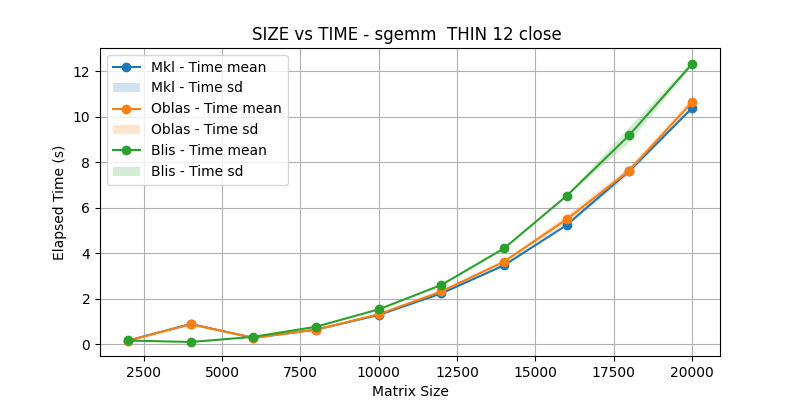
\includegraphics[width=\textwidth]{THIN 12/sgemm__THIN_12_close_time.png}
\end{figure}

As we can see, the MKL and OpenBLAS libraries are very similar in time terms while the BLIS library is a little bit slower for a size greater then 12000.

\begin{figure}[H]
    \centering
    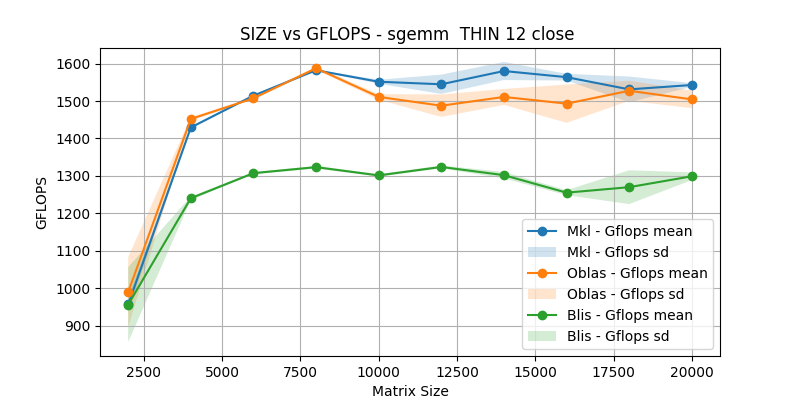
\includegraphics[width=\textwidth]{THIN 12/sgemm__THIN_12_close_gflops.png}
\end{figure}

As in the time study, the execution of the MKL and OpenBLAS libraries is similar, while the BLIS library allows to a smaller speed. In any case, we can see that with matrix sizes greater then 12000 we got a greater standard deviation in the experiments. 

 The plot below is still a test in single precision, but in this case we use the spread policy
\begin{figure}[H]
    \centering
    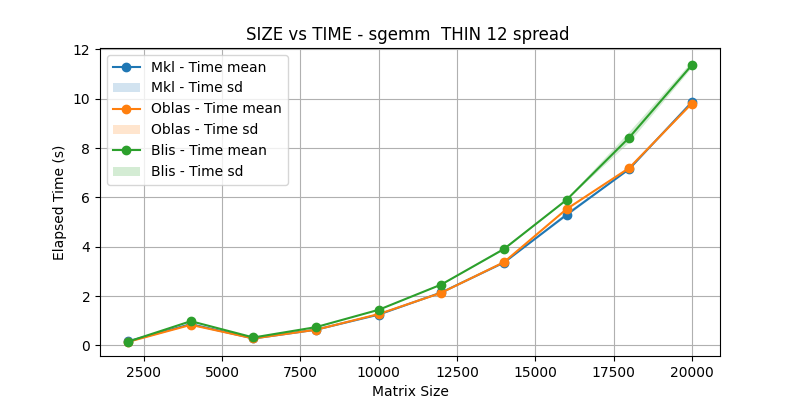
\includegraphics[width=\textwidth]{THIN 12/sgemm__THIN_12_spread_time.png}
\end{figure}

\begin{figure}[H]
    \centering
    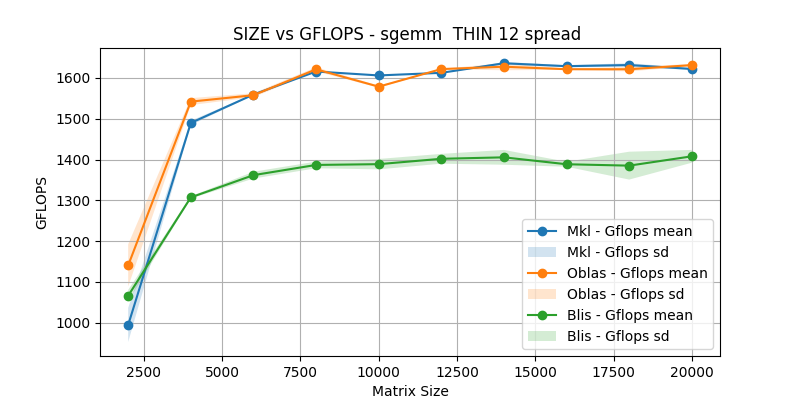
\includegraphics[width=\textwidth]{THIN 12/sgemm__THIN_12_spread_gflops.png}
\end{figure}

In times term, we have a similar results with respect to the close policy. However, it is interesting to see that the GFLOPS behavior of MKL and OpenBLAS in the spread case in much more similar w.r.t. the close policy.

Now, we repeated the previous tests, but in double precision.

\begin{figure}[H]
    \centering
    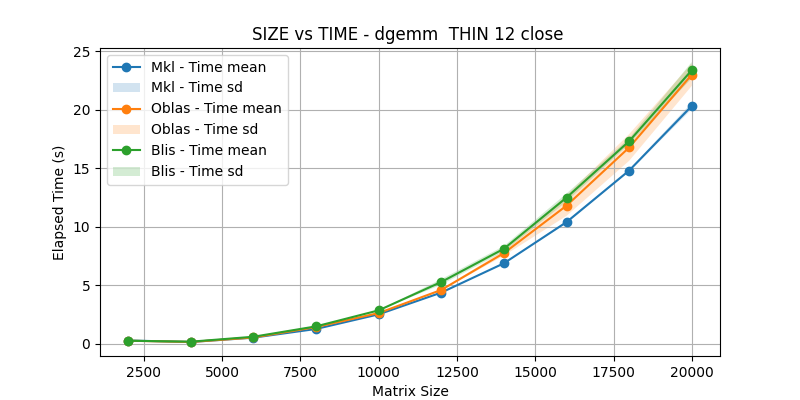
\includegraphics[width=\textwidth]{THIN 12/dgemm__THIN_12_close_time.png}
\end{figure}

\begin{figure}[H]
    \centering
    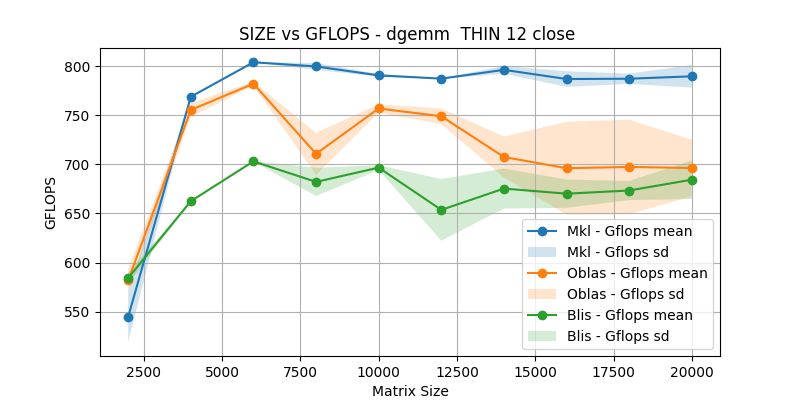
\includegraphics[width=\textwidth]{THIN 12/dgemm__THIN_12_close_gflops.png}
\end{figure}

In double precision the needed time is about twice the time of single precision, as we hoped, since it was coherent we our expectations. In this case, the greater speed was reached with the MKL library while with OpenBLAS the speed is similar to the blis one in case of big sizes. Furthermore, we can see the GFLOPS measures with OpenBLAS and BLIS have the biggest standard deviation seen w.r.t. all the previous cases studied.  

Finally, we tried the spread policy with double precision. In this case, we got a more clear behavior for the GFLOPS. As we can see in the following plots, the standard deviation is very small and we can state that the library with which we got the greater speed was MKL, followed by OpenBLAS, followed by BLIS.  

\begin{figure}[H]
    \centering
    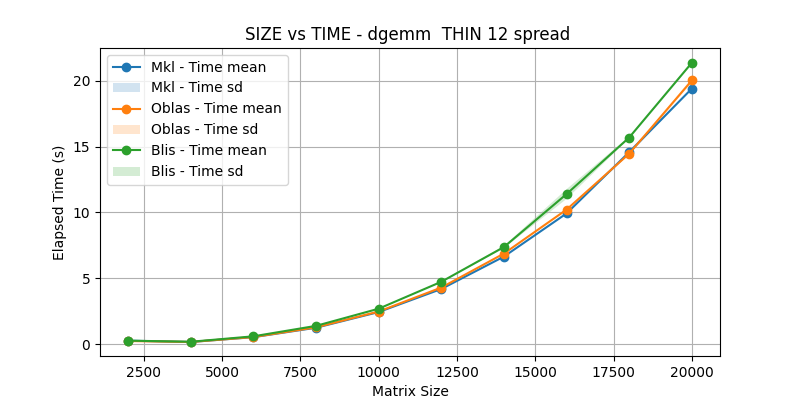
\includegraphics[width=\textwidth]{THIN 12/dgemm__THIN_12_spread_time.png}
\end{figure}

\begin{figure}[H]
    \centering
    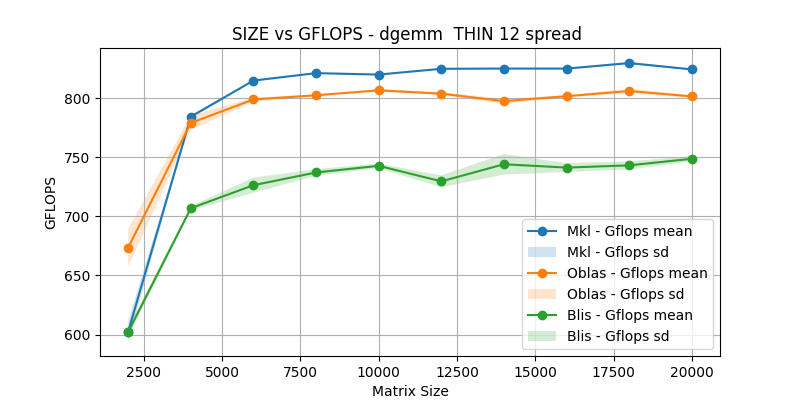
\includegraphics[width=\textwidth]{THIN 12/dgemm__THIN_12_spread_gflops.png}
\end{figure}



\subsubsection{Our peak performance}
The data:

With the THIN nodes, we reached the maximum performance in single precision with the MKL library on spread policy, when the size was 14000. The FLOPS were 1620.

For the double precision, we reached our maximum performance with MKL on spread policy, when the size was 18000. The FLOPS were 835. 

We concluded that, for the THIN nodes, with 12 cores, using spread policy and MKL library were the more important factors to reach the maximum performance. 

The optimized files: 

As we reported before, we try the command 
\begin{verbatim}
    -O3 -march=native
\end{verbatim}
in the compilation rules in order to increase the level of optimisation. Among all the trials, we chose to show the correspondent test on which in the previous files we reached the maximum performance so 
\begin{itemize}
    \item Single precision, spread policy
    \item Double precision, spread policy
\end{itemize}

For the single precision we can see that there is not a big difference.
\begin{figure}[H]
    \centering
    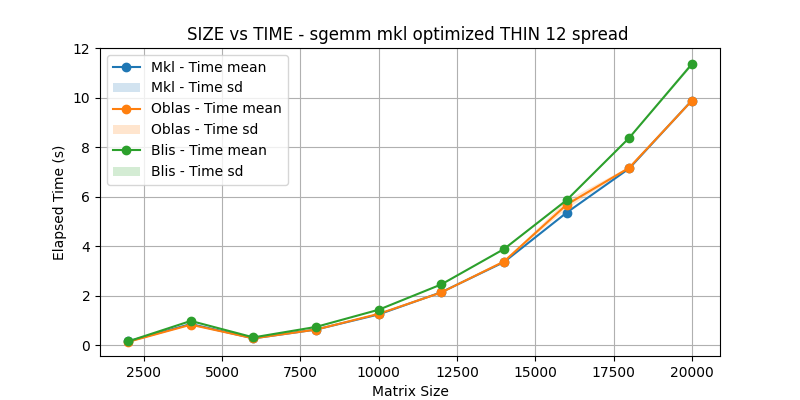
\includegraphics[width=\textwidth]{THIN 12/sgemm_mkl_optimized_THIN_12_spread_time.png}
\end{figure}

\begin{figure}[H]
    \centering
    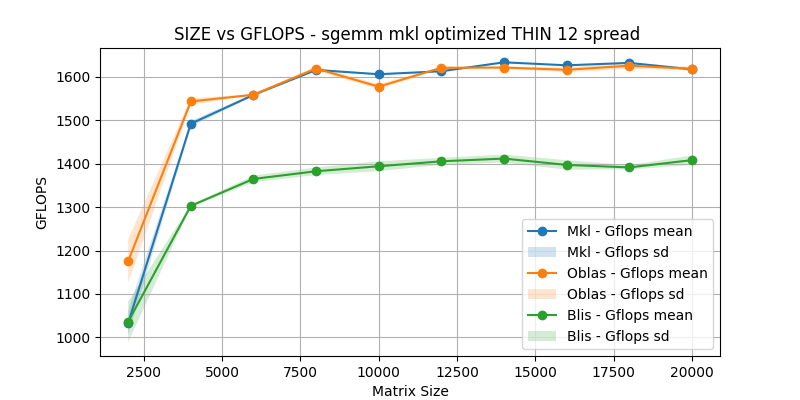
\includegraphics[width=\textwidth]{THIN 12/sgemm_mkl_optimized_THIN_12_spread_gflops.png}
\end{figure}

In the following plots, we plotted the results with the optimization steps. Here we can see that the GFLOPS are a little bit better then in the normal case but nothing special.  

\begin{figure}[H]
    \centering
    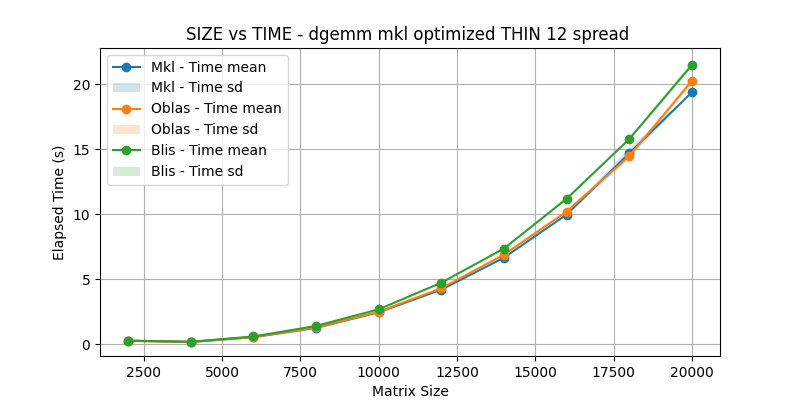
\includegraphics[width=\textwidth]{THIN 12/dgemm_mkl_optimized_THIN_12_spread_time.png}
\end{figure}

\begin{figure}[H]
    \centering
    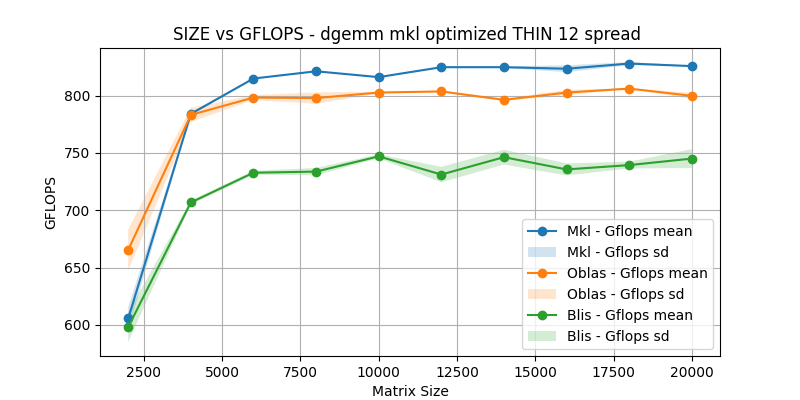
\includegraphics[width=\textwidth]{THIN 12/dgemm_mkl_optimized_THIN_12_spread_gflops.png}
\end{figure}

After the consideration of this section, we chose to omit the plots of the optimized libraries (they are in our GitHub anyway) since in the majority of the cases the were equal to the standard one and when they were better the improvement was very small.

\subsubsection{Results on fixed size}
In this sub subsection we will show our results regarding the strong scalability for the THIN nodes. As we discuss in the previous sections, our goal was to choose a size of the matrix in order to be enough big to appreciate the increase of speed when the used cores increases and sufficiently small to allow to an acceptable computation time. We had a threshold of 2 hours for each job, so we paid attention to avoid huge (relatively to our constraints) jobs. \
We chose a matrix size of 10000 and we increased the cpus from 1 to 24, by step of 2.
We started with close policy and single precision:
% Starting with "sgemm" and "close"
\begin{figure}[H]
    \centering
    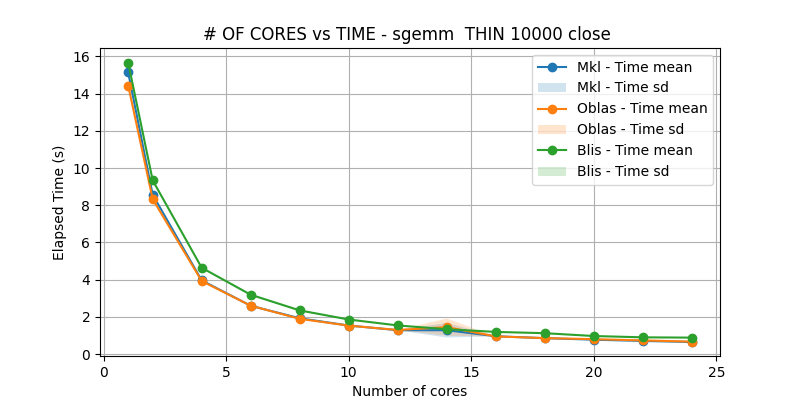
\includegraphics[width=\textwidth]{THIN scalability/sgemm__THIN_10000_close_time.png}
\end{figure}

\begin{figure}[H]
    \centering
    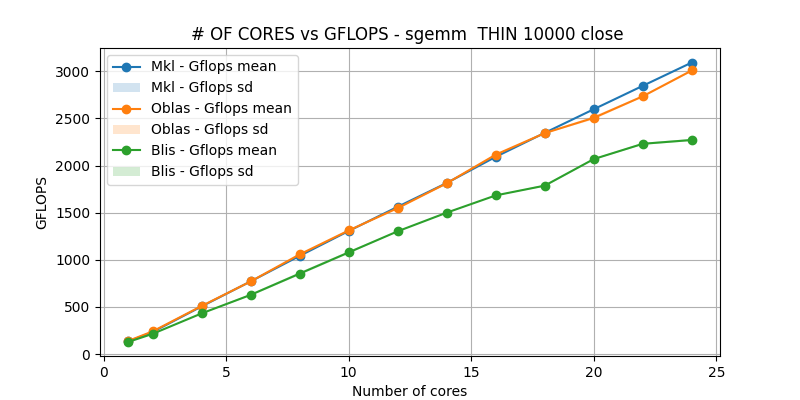
\includegraphics[width=\textwidth]{THIN scalability/sgemm__THIN_10000_close_gflops.png}
\end{figure}

We can see that the needed time drastically decreases when the cores go from 0 to 6. After 6 cores, the time continues to decrease, but more slowly. The GFLOPS have a clear linear growth on the number of cores.

% Replacing "close" with "spread"
Then, we did single precision tests with a spread policy.
\begin{figure}[H]
    \centering
    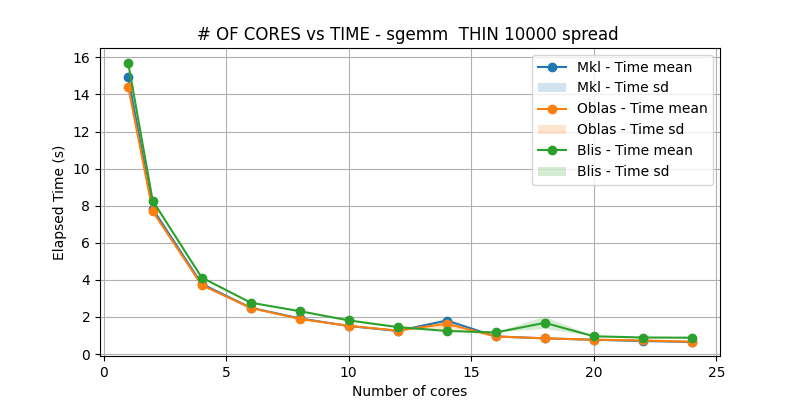
\includegraphics[width=\textwidth]{THIN scalability/sgemm__THIN_10000_spread_time.png}
\end{figure}

\begin{figure}[H]
    \centering
    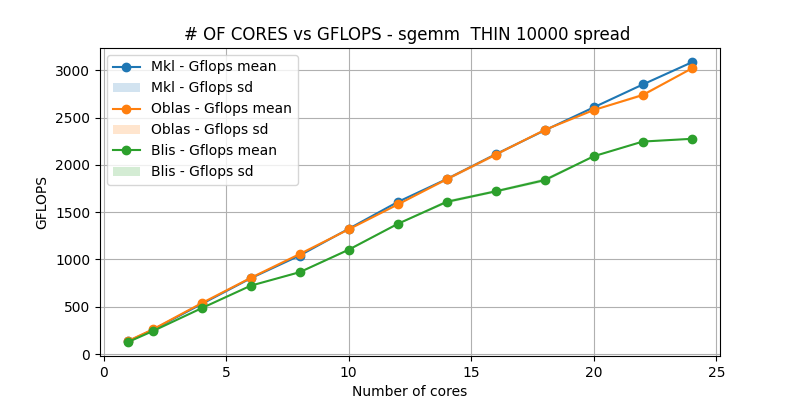
\includegraphics[width=\textwidth]{THIN scalability/sgemm__THIN_10000_spread_gflops.png}
\end{figure}

The results appears to be very similar to the close policy case. 

After, we tried the double precision.
% Replacing "sgemm" with "dgemm" and starting with "close"
\begin{figure}[H]
    \centering
    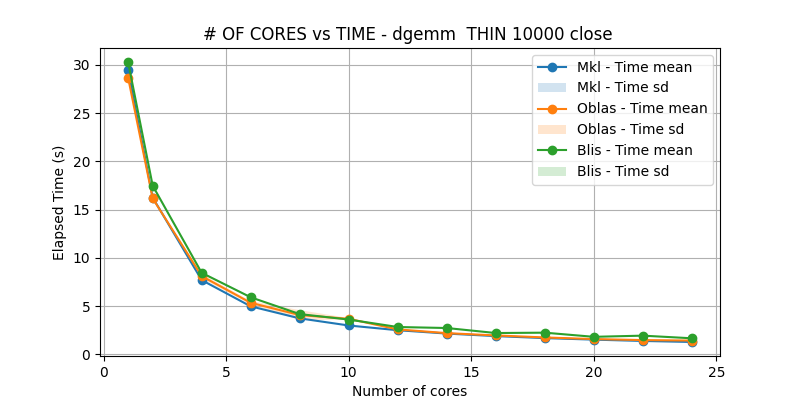
\includegraphics[width=\textwidth]{THIN scalability/dgemm__THIN_10000_close_time.png}
\end{figure}

\begin{figure}[H]
    \centering
    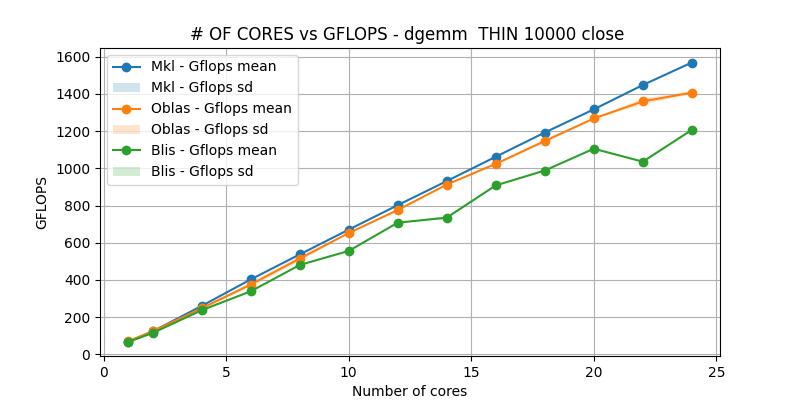
\includegraphics[width=\textwidth]{THIN scalability/dgemm__THIN_10000_close_gflops.png}
\end{figure}

Also in this case, we double the times w.r.t. single precision.

% spread
Finally, we tried the double precision with spread policy. As we can see in the following 2 plots all appears to be very similar to the previous case, but the behaviour of the GFLOPS in the BLIS case that is more regular.
\begin{figure}[H]
    \centering
    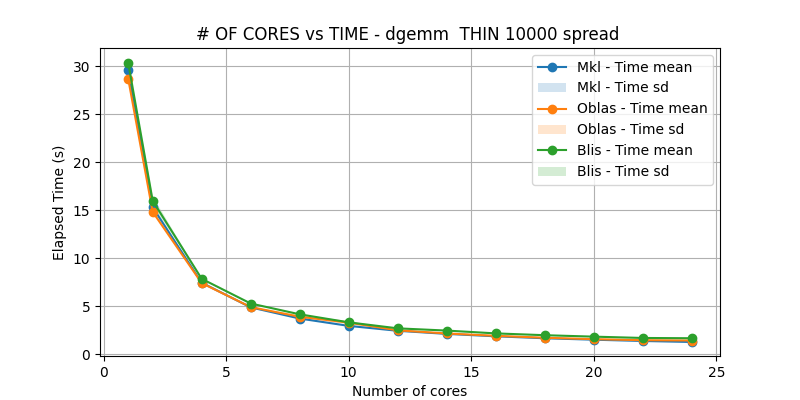
\includegraphics[width=\textwidth]{THIN scalability/dgemm__THIN_10000_spread_time.png}
\end{figure}

\begin{figure}[H]
    \centering
    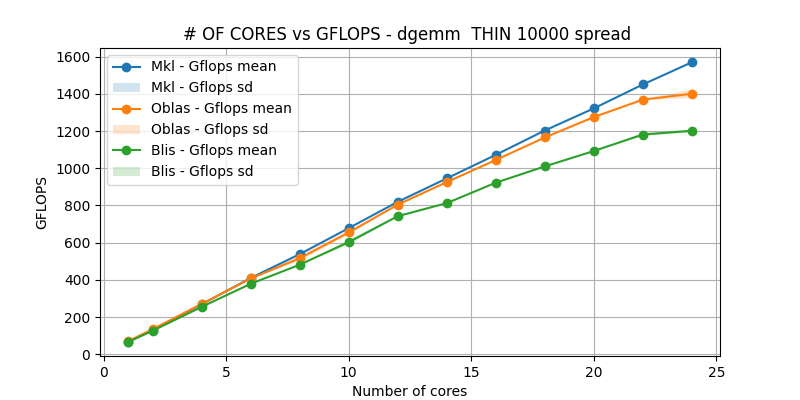
\includegraphics[width=\textwidth]{THIN scalability/dgemm__THIN_10000_spread_gflops.png}
\end{figure}

Now, since the big improvement of speed was from 1 to 6 cores, we focused on the range of cores from 1 to 10.

% Deep

% Starting with "sgemm" and "close"

We started with single precision and close policy. Differently from before, we can see in a clearer way the shape of the decrease of needed time when the used cores 
.   
\begin{figure}[H]
    \centering
    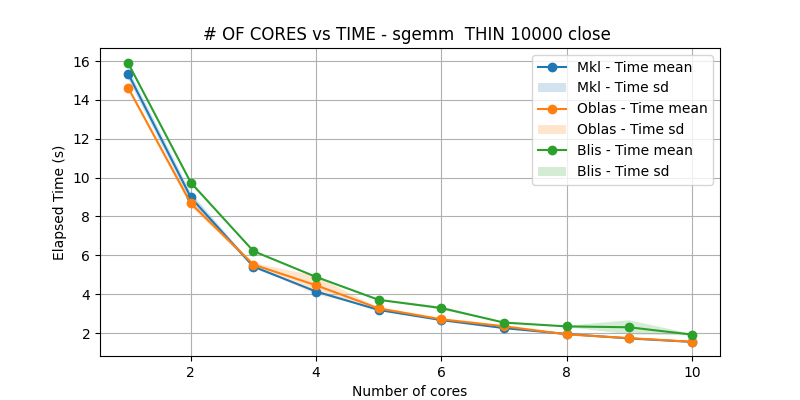
\includegraphics[width=\textwidth]{THIN scalability deep/sgemm__THIN_10000_close_time.png}
\end{figure}

\begin{figure}[H]
    \centering
    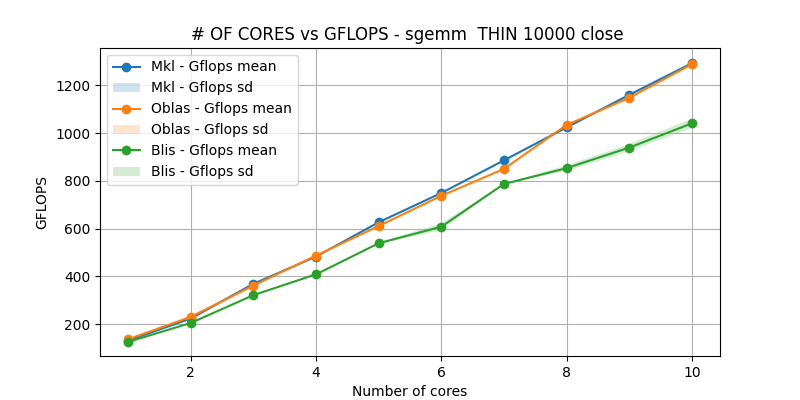
\includegraphics[width=\textwidth]{THIN scalability deep/sgemm__THIN_10000_close_gflops.png}
\end{figure}

% Replacing "close" with "spread"
Now we repeat the same thing, but with a spread policy.
\begin{figure}[H]
    \centering
    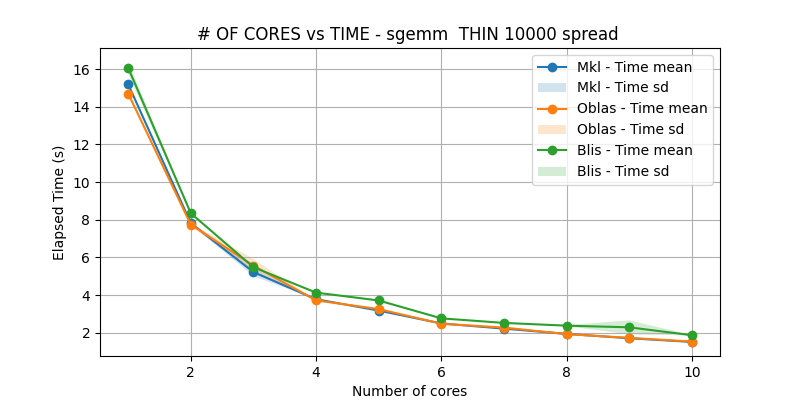
\includegraphics[width=\textwidth]{THIN scalability deep/sgemm__THIN_10000_spread_time.png}
\end{figure}

\begin{figure}[H]
    \centering
    \includegraphics[width=\textwidth]{THIN scalability deep/sgemm__THIN_10000_spread_gflops.png}
\end{figure}

% Replacing "sgemm" with "dgemm" and starting with "close"
Finally, we completed the THIN case by studying the time and GFLOPS behaviours when the cores increase from 1 to 10, by a step of 1.
\begin{figure}[H]
    \centering
    \includegraphics[width=\textwidth]{THIN scalability deep/dgemm__THIN_10000_close_time.png}
\end{figure}

\begin{figure}[H]
    \centering
    \includegraphics[width=\textwidth]{THIN scalability deep/dgemm__THIN_10000_close_gflops.png}
\end{figure}

% Replacing "close" with "spread"
\begin{figure}[H]
    \centering
    \includegraphics[width=\textwidth]{THIN scalability deep/dgemm__THIN_10000_spread_time.png}
\end{figure}

\begin{figure}[H]
    \centering
    \includegraphics[width=\textwidth]{THIN scalability deep/dgemm__THIN_10000_spread_gflops.png}
\end{figure}

\subsubsection{The speed up}
As we discussed before, the speed up is a function on the size and on the number of processors that is equal to the serial time over the parallel time with $p$ processors on a size $n$.
The ideal speed up is serialTime/parallelTime = serialTime/serialTime/$p$ = $p$, where $p$ is the number of processors used. Then, we hope to be the more close as possible to the function $f(x) = x $ in the plot cores $\times$ speedUp.

We tried the single precision on close and spread policy: 
\begin{figure}[H]
    \centering
    \includegraphics[width=\textwidth]{THIN speedUp/sgemm_mkl.x_THIN_10000_close_detailed__speedUp.png}
\end{figure}

\begin{figure}[H]
    \centering
    \includegraphics[width=\textwidth]{THIN speedUp/sgemm_mkl.x_THIN_10000_spread_detailed__speedUp.png}
\end{figure}

As we can see we are really close to the ideal speed up and it's a great thing. Especially the MKL library is the best.

Then, we tested the speed up for the double precision. The following plots shows that we have a situation simlar to the single precision. The MKL library continue to be the best in speed up term since it is very close to the ideal speed up.

Close policy:
\begin{figure}[H]
    \centering
    \includegraphics[width=\textwidth]{THIN speedUp/dgemm_mkl.x_THIN_10000_close_detailed__speedUp.png}
\end{figure}

Spread policy:
\begin{figure}[H]
    \centering
    \includegraphics[width=\textwidth]{THIN speedUp/dgemm_mkl.x_THIN_10000_spread_detailed__speedUp.png}
\end{figure}

\subsection{EPYC case}
We tested the EPYC nodes and reported the results on this section. The schema was very similar to the previous section, but with a different focus on cores range in the strong scalability study. 

\subsubsection{Results on fixed number of cores}
An EPYC node has 128 cores in 2 sockets. Then we fixed a number of cores different from the THIN tests (now we used 64) and repeated the experiments for the MKL, OpenBLAS and BLIS libraries.   

First of all, we tested the three libraries with single precision and close policy.
\begin{figure}[H]
    \centering
    \includegraphics[width=\textwidth]{EPYC 64/sgemm__EPYC_64_close_time.png}
\end{figure}

\begin{figure}[H]
    \centering
    \includegraphics[width=\textwidth]{EPYC 64/sgemm__EPYC_64_close_gflops.png}
\end{figure}

It is very interesting to see that in this case the worst library, both in time and GFLOPS terms, is MKL. On the other hand, OpenBLAS is the best. In the THIN case the OpenBLAS was worse or close to the MKL. There is a big standard deviation, maybe because we did only 5 iterations for each size (instead of the 10 of the THIN nodes). 

In the following plots we tested the spread policy. 
\begin{figure}[H]
    \centering
    \includegraphics[width=\textwidth]{EPYC 64/sgemm__EPYC_64_spread_time.png}
\end{figure}

\begin{figure}[H]
    \centering
    \includegraphics[width=\textwidth]{EPYC 64/sgemm__EPYC_64_spread_gflops.png}
\end{figure}

The spread case differs from the close case by a strange behaviours of the GFLOPS for the MKL and BLIS libraries and a clear and almost linear increase of GFLOPS for the OpenBLAS library. 

The, we tested the EPYC nodes with double precision. We started with a close policy.
\begin{figure}[H]
    \centering
    \includegraphics[width=\textwidth]{EPYC 64/dgemm__EPYC_64_close_time.png}
\end{figure}

\begin{figure}[H]
    \centering
    \includegraphics[width=\textwidth]{EPYC 64/dgemm__EPYC_64_close_gflops.png}
\end{figure}

It is notable that the blue line outperforms the red and blue lines (especially in GFLOPS terms). So, we found a case where the BLIS library appears to be the better. 

In order to conclude this sub section, we will show the case of double precision and spread policy. 
The graph illustrates similar times. The MKL appears to be a little bit better, but it has a greater standard deviation. 
\begin{figure}[H]
    \centering
    \includegraphics[width=\textwidth]{EPYC 64/dgemm__EPYC_64_spread_time.png}
\end{figure}

\begin{figure}[H]
    \centering
    \includegraphics[width=\textwidth]{EPYC 64/dgemm__EPYC_64_spread_gflops.png}
\end{figure}

The data shows a steady domain of the BLIS library in GFLOPS terms. 

\subsubsection{Our peak performance}
For the EPYC nodes, we reached our peak performance for the single precision with the BLIS library and spread policy. Our peak performance was 2750 GFLOPS.

While, for the double precision, the peak performance was reached with BLIS library and close policy (1180 GFLOPS). We have to mention that with BLIS library and spread policy we were just a little bit below the 1180 GFLOPS, but we had a large standard deviation.

In any case, we can say that for the EPYC node the BLIS library is the best in order to reach the maximum performance. 

\subsubsection{Results on fixed size}
In this sub subsection we tested the strong scalability with the EPYC nodes. We fix a size of the matrix of 10000 in order to be consistent to the THIN studies. We increased the number of cores from 1 to 128 by steps of 16. We did more measures in the $[1,16]$ cores range, since is there then the time decreases the more.  

% Starting with "sgemm" and "close"
As usual, we started with single precision and close policy. 
\begin{figure}[H]
    \centering
    \includegraphics[width=\textwidth]{EPYC scalability/sgemm__EPYC_10000_close_time.png}
\end{figure}

\begin{figure}[H]
    \centering
    \includegraphics[width=\textwidth]{EPYC scalability/sgemm__EPYC_10000_close_gflops.png}
\end{figure}
In the chart, we can see an immediate and sudden decrease of execution time. While we observe a peak of GFLOPS when the number of cores is around 40. 

% Replacing "close" with "spread"
We did the same tests, but with spread policy.
\begin{figure}[H]
    \centering
    \includegraphics[width=\textwidth]{EPYC scalability/sgemm__EPYC_10000_spread_time.png}
\end{figure}

\begin{figure}[H]
    \centering
    \includegraphics[width=\textwidth]{EPYC scalability/sgemm__EPYC_10000_spread_gflops.png}
\end{figure}
In contrast to the close policy,the spread policy exhibits a lower pick of performance of the OpenBLAS library. 

% Replacing "sgemm" with "dgemm" and starting with "close"
After, we tried the double precision.
\begin{figure}[H]
    \centering
    \includegraphics[width=\textwidth]{EPYC scalability/dgemm__EPYC_10000_close_time.png}
\end{figure}

\begin{figure}[H]
    \centering
    \includegraphics[width=\textwidth]{EPYC scalability/dgemm__EPYC_10000_close_gflops.png}
\end{figure}

It is interesting to note that the MKL library is worse then the others in both times and GFLOPS terms.

% Replacing "close" with "spread"
This plot presents data on the spread policy.
\begin{figure}[H]
    \centering
    \includegraphics[width=\textwidth]{EPYC scalability/dgemm__EPYC_10000_spread_time.png}
\end{figure}

\begin{figure}[H]
    \centering
    \includegraphics[width=\textwidth]{EPYC scalability/dgemm__EPYC_10000_spread_gflops.png}
\end{figure}
In this case, there is a clear upward trend of the BLIS library.

In order to conclude the EPYC study, we wanted to focused on the $[1,16]$ range for the cores.
This plot presents data on single precision with close policy.
% Starting with "sgemm" and "close"
\begin{figure}[H]
    \centering
    \includegraphics[width=\textwidth]{EPYC scalability deep/sgemm__EPYC_10000_close_time.png}
\end{figure}

\begin{figure}[H]
    \centering
    \includegraphics[width=\textwidth]{EPYC scalability deep/sgemm__EPYC_10000_close_gflops.png}
\end{figure}
Now there is a clearer view of the worse performance of the MKL library. 

% Replacing "close" with "spread"
We got similar result for the spread policy.
\begin{figure}[H]
    \centering
    \includegraphics[width=\textwidth]{EPYC scalability deep/sgemm__EPYC_10000_spread_time.png}
\end{figure}

\begin{figure}[H]
    \centering
    \includegraphics[width=\textwidth]{EPYC scalability deep/sgemm__EPYC_10000_spread_gflops.png}
\end{figure}

% Replacing "sgemm" with "dgemm" and starting with "close"
The figure provides an overview of the tests on double precision.
\begin{figure}[H]
    \centering
    \includegraphics[width=\textwidth]{EPYC scalability deep/dgemm__EPYC_10000_close_time.png}
\end{figure}

\begin{figure}[H]
    \centering
    \includegraphics[width=\textwidth]{EPYC scalability deep/dgemm__EPYC_10000_close_gflops.png}
\end{figure}

In this case, there appears to be a similarity between the three libraries.

% Replacing "close" with "spread"
A really analogous behaviour in the spread policy cases.
\begin{figure}[H]
    \centering
    \includegraphics[width=\textwidth]{EPYC scalability deep/dgemm__EPYC_10000_spread_time.png}
\end{figure}

\begin{figure}[H]
    \centering
    \includegraphics[width=\textwidth]{EPYC scalability deep/dgemm__EPYC_10000_spread_gflops.png}
\end{figure}



\end{document}